\renewcommand{\theequation}{\theenumi}
\begin{enumerate}[label=\arabic*.,ref=\thesubsection.\theenumi]
\numberwithin{equation}{enumi}
\item  Equal chords of a circle (or of congruent circles) subtend equal angles at the centre. 
\item  If the angles subtended by two chords of a circle (or of congruent circles) at the centre (corresponding centres) are equal, the chords are equal.
\item  The perpendicular from the centre of a circle to a chord bisects the chord. 
\item  The line drawn through the centre of a circle to bisect a chord is perpendicular to the chord.
\item  There is one and only one circle passing through three non-collinear points. 
\item  Equal chords of a circle (or of congruent circles) are equidistant from the centre (or corresponding centres).
\item Chords equidistant from the centre (or corresponding centres) of a circle (or of congruent circles) are equal.
\item  If two arcs of a circle are congruent, then their corresponding chords are equal and conversely if two chords of a circle are equal, then their corresponding arcs (minor, major) are congruent.
\item Congruent arcs of a circle subtend equal angles at the centre. 
\item  The angle subtended by an arc at the centre is double the angle subtended by it at any point on the remaining part of the circle.
\item Angles in the same segment of a circle are equal. \item  Angle in a semicircle is a right angle. 
\item  If a line segment joining two points subtends equal angles at two other points lying on the same side of the line containing the line segment, the four points lie on a circle. 
\begin{enumerate}

%\renewcommand{\thefigure}{\theenumi.\arabic{figure}}
\begin{figure}[!ht]
\centering
\resizebox{\columnwidth}{!}{\renewcommand{\theequation}{\theenumi}
\begin{enumerate}[label=\thesection.\arabic*.,ref=\thesection.\theenumi]
\numberwithin{equation}{enumi}
\item  Find the centre and radius of the circle 
\begin{align}
x^2+y^2+8x+10y-8 = 0
\label{eq:circ_basic}
\end{align}
\solution
\eqref{eq:circ_basic} can be expressed as 
\begin{align}
\vec{x}^T\vec{x}+ 2\myvec{4 & 5}\vec{x} -8 = 0
\end{align}
which is of the form \eqref{eq:conic_quad_form} with
\begin{align}
\label{eq:circ_basic_uf}
\vec{u} = \myvec{4\\5}, f = -8
\end{align}
From  Table \ref{table:conics}, the center and radius are given by 
\begin{align}
\vec{c} = -\vec{u} = \myvec{-4\\-5},
r = \sqrt{\norm{u}^2-f} = 7
\end{align}
\item Find the equation of a circle which passes through the points $\vec{P} = \myvec{2\\-2}$ and $\vec{Q} = \myvec{3\\4}$ and whose centre lies on the line  
%\cite{eleven}
\begin{align}
\label{eq:circ_ex1_line}
\myvec{1 & 1} \vec{x} = 2
\end{align}
\solution From \eqref{eq:conic_quad_form} and Table \ref{table:conics}, the equation of a circle can be expressed as
\begin{align}
\label{eq:circ_conic}
\vec{x}^T\vec{x}-2\vec{c}^T\vec{x}+f = 0
\end{align}
where $\vec{c}$ is the centre.
Substituting the given points in 
\eqref{eq:circ_conic} and using 
\eqref{eq:circ_ex1_line}, the following equations are obtained
\begin{align}
2\myvec{2 & -2}\vec{c} -  f &= 8
\\
2\myvec{3 & 4}\vec{c} -  f &= 25
\\
\myvec{1 & 1}\vec{c}  &= 2
\end{align}
which can be expressed as the matrix equation
\begin{align}
\myvec{
1 & 1 & 0
\\
4 & -4 & -1 
\\ 
6 & 8 & -1  
}
\myvec{\vec{c}\\f} = \myvec{2\\8\\25}
\end{align}
Row reducing the augmented matrix
\begin{align}
\myvec{
1 & 1 & 0 & 2
\\
4 & -4 & -1 & 8
\\ 
6 & 8 & -1  & 25
}
\\
\xleftrightarrow[R_3 \leftarrow R_3 -6R_1]{R_2 \leftarrow -R_2+4R_1}
\myvec{
1 & 1 & 0 & 2
\\
0 & 8 & 1 & 0
\\ 
0 & 2 & -1  & 13
}
\\
\xleftrightarrow[R_3 \leftarrow -\frac{4R_3 -R_2}{2}]{R_1 \leftarrow 8R_1-R_3}
\myvec{
8 & 0 & -1 & 16
\\
0 & 8 & 1 & 0
\\ 
0 & 0 & 5  & -52
}
\\
\xleftrightarrow[R_2 \leftarrow \frac{5R_2 -R_3}{4}]{R_1 \leftarrow \frac{5R_1+R_3}{4}}
\myvec{
10 & 0 & 0 & 7
\\
0 & 10 & 0 & 13
\\ 
0 & 0 & 5  & -52
}
\end{align}
Thus, 
\begin{align}
\vec{c} &= \frac{1}{10}\myvec{7\\13}
\\
f &=-\frac{52}{5}
\end{align}
which give the desired equation of the circle.
From Table \ref{table:conics},
%
\begin{align}
 r =  \sqrt{\norm{\vec{c}}^2-f} = \frac{1}{10}\sqrt{1258}
\end{align}
Fig. \ref{fig:CircOr}	verifies the above results.

\begin{figure}[!ht]
\centering
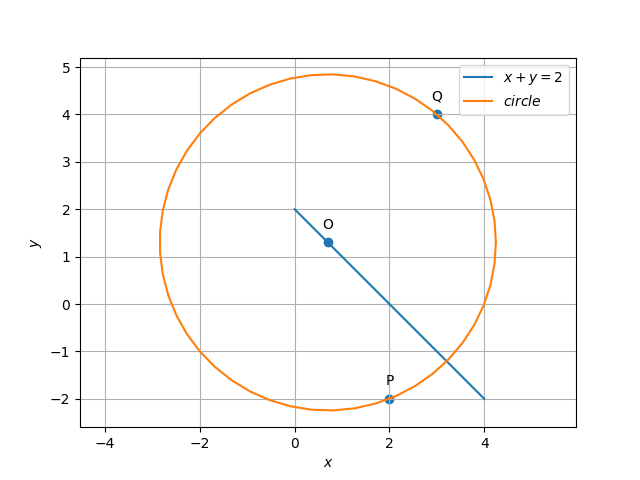
\includegraphics[width=\columnwidth]{./figs/circex/CircOr.eps}
\caption{Circle passing through $\myvec{2\\-2},\myvec{3\\4}$. Center is on line $\myvec{1 & 1}\vec{x}=2$. }
\label{fig:CircOr}	
\end{figure}

\item 
Find the points on the curve  
%\cite{twelve_one}
\begin{align}
x^2+y^2-2x-3 = 0
\label{eq:circle_tangent_prob}
\end{align}
at which the tangents are parallel to the $x$-axis.
\\
\solution \eqref{eq:circle_tangent_prob} can be expressed as
\begin{align}
\vec{x}^T\vec{x}+\myvec{-2 & 0}\vec{x}-3 &= 0
\label{eq:circle_tangent_prob_vec}
\\
\implies \vec{V} = \vec{I}, \vec{u} = \myvec{-1 \\ 0}, f = -3
\label{eq:circle_tangent_prob_uf}
\end{align}
From Table \ref{table:conics}, the centre and radius are
\begin{align}
\vec{c} = -\vec{u} = \myvec{-1 \\ 0}, r =\sqrt{\norm{\vec{u}}^2-f} = 2
\end{align}
$\because$ the tangents are parallel to the $x$-axis, their direction and normal vectors are respectively,
\begin{align}
\vec{m} = \myvec{1\\0},
\vec{n} = \myvec{0\\1}.
\end{align}
From Table \ref{table:conics},
\begin{align}
\kappa = \pm \sqrt{\frac{\vec{u}^T\vec{u}-f}{\vec{n}^T\vec{n}}} = \pm \sqrt{\frac{4}{1}} = \pm 2
\end{align}
and the desired points of contact are 
\begin{align}
\vec{q}_1, \vec{q}_2 = \myvec{1\\0}\pm 2\myvec{0\\1} =  
\myvec{1 \\  2},
\myvec{1 \\  -2}
\end{align}
%
Fig. \ref{fig:CircOr}	verifies the above results.
\begin{figure}[!ht]
\centering
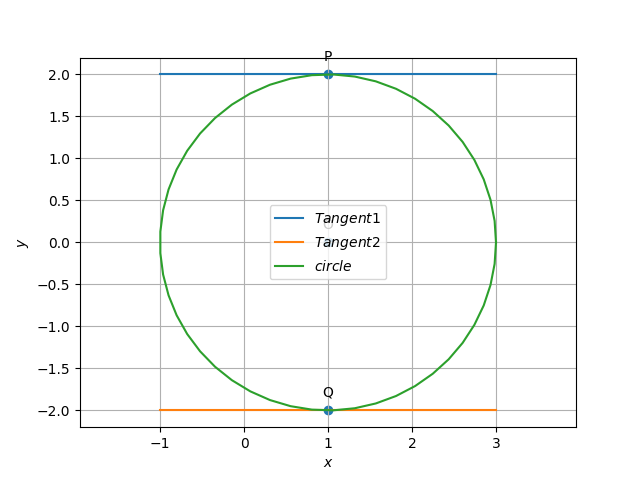
\includegraphics[width=\columnwidth]{./figs/circex/CircTangent.eps}
\caption{Tangents are parallel to the $x$-axis. }
\label{fig:CircTangent}	
\end{figure}

\end{enumerate}
}
\caption{}
\label{fig:8.5.16_circle_latex}	
\end{figure}
%
%
%\renewcommand{\thefigure}{\theenumi}
%
\item {\em Construction: }In Fig. \ref{fig:8.5.16_circle_latex} the known parameters are
%\label{}
\\
%
%\solution From the given information, 
%$\triangle ABC$ are 
\begin{align}
\vec{O} &= \myvec{0\\0} ,
\\
\vec{A} &= \myvec{r\\0} ,
\label{eq:8.5.16_constr_a}
\\
 \vec{B} &= \myvec{-r\\0} 
\label{eq:8.5.16_constr_b}
\\
\vec{C}&= r\myvec{\cos\theta\\\sin\theta}
\label{eq:8.5.16_constr_cgen}
\end{align}
%
Let 
\begin{align}
\vec{D} & = r\myvec{\cos\theta_1\\\sin\theta_1} 
\label{eq:8.5.16_constr_dgen}
\end{align}
From the given information,
\begin{align}
 \norm{\vec{D} - \vec{C}} &= r
\\
\implies \brak{\vec{D} - \vec{C}}^T\brak{\vec{D} - \vec{C}} &= r^2\\
 \label{eq:8.5.16_dist_formula}
\\
\implies  \norm{D} ^2 - 2\vec{D}^T\vec{C} +  \norm{C}^2 &=r^2 
\end{align}
In the above, 
\begin{align}
\because \norm{D} &= \norm{\vec{C}} = r,
\\
\frac{\vec{D}^T\vec{C}}{\norm{D}\norm{C}}  &= \frac{1}{2}
\\
\implies \cos \brak{\theta_1-\theta} &= 60 \degree
\label{eq:8.5.16_theta_diff}
\end{align}
using the definition of the inner product.  $\because \theta$ is known, we get $\theta_1$ from \eqref{eq:8.5.16_theta_diff}
and $\vec{D}$ from 
\eqref{eq:8.5.16_constr_dgen}. 
%
\subitem Thus,
\begin{align}
BD: \vec{x} &= \vec{B} + \lambda_1 \brak{\vec{B}-\vec{D}}
\\
AC: \vec{x} &= \vec{A} + \lambda_2 \brak{\vec{A}-\vec{C}}
\end{align}
%
which can be used to obtain $\vec{E}$.



General equation of conics is 
\begin{align}
    \vec{x}^T\vec{V}\vec{x}+ 2\vec{u}^T\vec{x}+f = 0
    \label{eq:solutions/1/16/eq:1}
\end{align}
Comparing with the equation given,
\begin{align}
\vec{V}=\myvec{\frac{1}{9} & 0 \\ 0 & \frac{1}{16}}\\
\vec{u}=\vec{0}\\
f=-1\\
\mydet{\vec{v}}=\mydet{\myvec{\frac{1}{9} & 0 \\ 0 & \frac{1}{16}}}>0
\end{align}
$\because \abs{\vec{V}}>0$, the given equation is of ellipse.\\
a)The tangents are parallel to the x-axis, hence, their direction and normal vectors, $\vec{m_1}$ and $\vec{n_1}$ are respectively,
\begin{align}
\vec{m_1}=\myvec{1\\0}\\
\vec{n_1}=\myvec{0\\1}
\end{align}
For an ellipse, given the normal vector $\vec{n}$, the tangent points of contact to the ellipse are given by
\begin{align}
    \vec{q}=\vec{V}^{-1}(\kappa \vec{n}-\vec{u})
    \label{eq:solutions/1/16/eq:2}
    =\vec{V}^{-1}\kappa \vec{n}
\end{align}
where
\begin{align}
    \kappa=\pm \sqrt{\frac{\vec{u^T}\vec{V}^{-1}\vec{u}-f}{\vec{n^T}\vec{V}^{-1}\vec{n}}}
    \label{eq:solutions/1/16/eq:2.0.9}\\
   =\pm \sqrt{\frac{-f}{\vec{n^T}\vec{V}^{-1}\vec{n}}}\\
    \vec{V}^{-1}=\myvec{9 & 0 \\ 0 & 16}\\
    \kappa_1=\pm \sqrt{\frac{-(-1)}{\myvec{0 & 1}\myvec{9 & 0 \\ 0 & 16} \myvec{0\\1}}}\\
 \implies \kappa_1=\pm \sqrt{\frac{1}{16}}\\
    \implies \kappa_1=\pm \frac{1}{4}      
\end{align}
From \eqref{eq:solutions/1/16/eq:2} , the point of contact $\vec{q_i}$ are,
\begin{align}
    \vec{q_1}=\myvec{9 & 0 \\ 0 & 16}\frac{1}{4}\myvec{0\\1}\\
    =\myvec{9 & 0 \\ 0 & 16}\myvec{0\\\frac{1}{4}}\\
    =\myvec{0\\4}\\
    \vec{q_2}=\myvec{9 & 0 \\ 0 & 16}\left(-\frac{1}{4}\right)\ \myvec{0\\1}\\
    =\myvec{9 & 0 \\ 0 & 16}\myvec{0\\-\frac{1}{4}}\\
    =\myvec{0\\-4}
\end{align}
b) The tangents are parallel to the y-axis, hence, their direction and normal vectors, $\vec{m_2}$ and $\vec{n_2}$ are respectively,
\begin{align}
\vec{m_2}=\myvec{0\\1}\\
\vec{n_2}=\myvec{1\\0}
\end{align}
Using equation \eqref{eq:solutions/1/16/eq:2.0.9}, the values of $\kappa$ for this case are
\begin{align}
     \kappa_2=\pm \sqrt{\frac{-(-1)}{\myvec{1 & 0}\myvec{9 & 0 \\ 0 & 16} \myvec{1\\0}}}\\
 \implies \kappa_2=\pm \sqrt{\frac{1}{9}}\\
    \implies \kappa_2=\pm \frac{1}{3} 
\end{align}
and from \eqref{eq:solutions/1/16/eq:2} , the point of contact $\vec{q_i}$ are,
\begin{align}
\vec{q_3}=\myvec{9 & 0 \\ 0 & 16}\frac{1}{3}\myvec{1\\0}\\
    =\myvec{9 & 0 \\ 0 & 16}\myvec{\frac{1}{3}\\0}\\
    =\myvec{3\\0}\\
\vec{q_4}=\myvec{9 & 0 \\ 0 & 16}\left(-\frac{1}{3}\right)\ \myvec{1\\0}\\
    =\myvec{9 & 0 \\ 0 & 16}\myvec{-\frac{1}{3}\\0}\\
    =\myvec{-3\\0}
\end{align}
 \begin{figure}[h!]
	\centering
	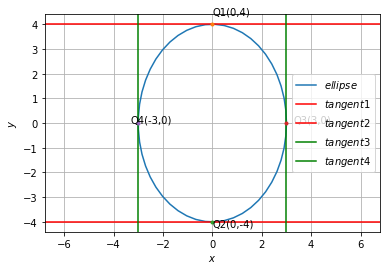
\includegraphics[width=\columnwidth]{./solutions/conics/1/16/ellipse.png}
	\caption{Figure depicting point of contact of tangents of ellipse parallel to x-axis and y-axis}
	\label{eq:solutions/1/16/fig1}
\end{figure}

\end{enumerate}
\item  The sum of either pair of opposite angles of a cyclic quadrilateral is 180$\degree$.
\item  If sum of a pair of opposite angles of a quadrilateral is 180$\degree$, the quadrilateral is cyclic.
%
\item AB is a diameter of the circle, $CD$ is a chord equal to the radius of the circle. $AC$ and $BD$ when extended intersect at a point $E$. Prove that $\angle AEB = 60\degree$.
\begin{enumerate}

%\renewcommand{\thefigure}{\theenumi.\arabic{figure}}
\begin{figure}[!ht]
\centering
\resizebox{\columnwidth}{!}{\renewcommand{\theequation}{\theenumi}
\begin{enumerate}[label=\thesection.\arabic*.,ref=\thesection.\theenumi]
\numberwithin{equation}{enumi}
\item  Find the centre and radius of the circle 
\begin{align}
x^2+y^2+8x+10y-8 = 0
\label{eq:circ_basic}
\end{align}
\solution
\eqref{eq:circ_basic} can be expressed as 
\begin{align}
\vec{x}^T\vec{x}+ 2\myvec{4 & 5}\vec{x} -8 = 0
\end{align}
which is of the form \eqref{eq:conic_quad_form} with
\begin{align}
\label{eq:circ_basic_uf}
\vec{u} = \myvec{4\\5}, f = -8
\end{align}
From  Table \ref{table:conics}, the center and radius are given by 
\begin{align}
\vec{c} = -\vec{u} = \myvec{-4\\-5},
r = \sqrt{\norm{u}^2-f} = 7
\end{align}
\item Find the equation of a circle which passes through the points $\vec{P} = \myvec{2\\-2}$ and $\vec{Q} = \myvec{3\\4}$ and whose centre lies on the line  
%\cite{eleven}
\begin{align}
\label{eq:circ_ex1_line}
\myvec{1 & 1} \vec{x} = 2
\end{align}
\solution From \eqref{eq:conic_quad_form} and Table \ref{table:conics}, the equation of a circle can be expressed as
\begin{align}
\label{eq:circ_conic}
\vec{x}^T\vec{x}-2\vec{c}^T\vec{x}+f = 0
\end{align}
where $\vec{c}$ is the centre.
Substituting the given points in 
\eqref{eq:circ_conic} and using 
\eqref{eq:circ_ex1_line}, the following equations are obtained
\begin{align}
2\myvec{2 & -2}\vec{c} -  f &= 8
\\
2\myvec{3 & 4}\vec{c} -  f &= 25
\\
\myvec{1 & 1}\vec{c}  &= 2
\end{align}
which can be expressed as the matrix equation
\begin{align}
\myvec{
1 & 1 & 0
\\
4 & -4 & -1 
\\ 
6 & 8 & -1  
}
\myvec{\vec{c}\\f} = \myvec{2\\8\\25}
\end{align}
Row reducing the augmented matrix
\begin{align}
\myvec{
1 & 1 & 0 & 2
\\
4 & -4 & -1 & 8
\\ 
6 & 8 & -1  & 25
}
\\
\xleftrightarrow[R_3 \leftarrow R_3 -6R_1]{R_2 \leftarrow -R_2+4R_1}
\myvec{
1 & 1 & 0 & 2
\\
0 & 8 & 1 & 0
\\ 
0 & 2 & -1  & 13
}
\\
\xleftrightarrow[R_3 \leftarrow -\frac{4R_3 -R_2}{2}]{R_1 \leftarrow 8R_1-R_3}
\myvec{
8 & 0 & -1 & 16
\\
0 & 8 & 1 & 0
\\ 
0 & 0 & 5  & -52
}
\\
\xleftrightarrow[R_2 \leftarrow \frac{5R_2 -R_3}{4}]{R_1 \leftarrow \frac{5R_1+R_3}{4}}
\myvec{
10 & 0 & 0 & 7
\\
0 & 10 & 0 & 13
\\ 
0 & 0 & 5  & -52
}
\end{align}
Thus, 
\begin{align}
\vec{c} &= \frac{1}{10}\myvec{7\\13}
\\
f &=-\frac{52}{5}
\end{align}
which give the desired equation of the circle.
From Table \ref{table:conics},
%
\begin{align}
 r =  \sqrt{\norm{\vec{c}}^2-f} = \frac{1}{10}\sqrt{1258}
\end{align}
Fig. \ref{fig:CircOr}	verifies the above results.

\begin{figure}[!ht]
\centering
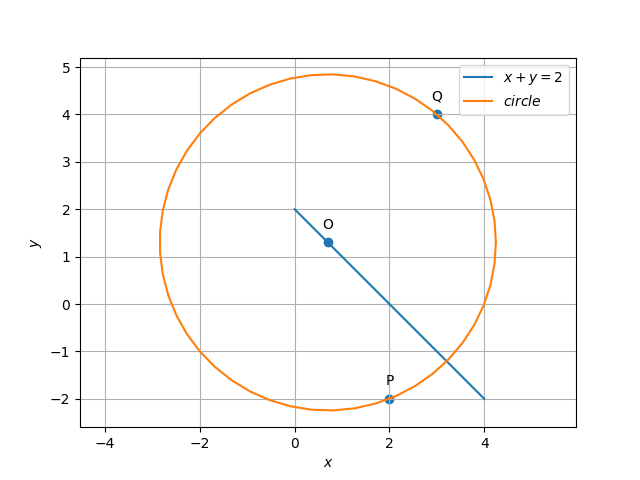
\includegraphics[width=\columnwidth]{./figs/circex/CircOr.eps}
\caption{Circle passing through $\myvec{2\\-2},\myvec{3\\4}$. Center is on line $\myvec{1 & 1}\vec{x}=2$. }
\label{fig:CircOr}	
\end{figure}

\item 
Find the points on the curve  
%\cite{twelve_one}
\begin{align}
x^2+y^2-2x-3 = 0
\label{eq:circle_tangent_prob}
\end{align}
at which the tangents are parallel to the $x$-axis.
\\
\solution \eqref{eq:circle_tangent_prob} can be expressed as
\begin{align}
\vec{x}^T\vec{x}+\myvec{-2 & 0}\vec{x}-3 &= 0
\label{eq:circle_tangent_prob_vec}
\\
\implies \vec{V} = \vec{I}, \vec{u} = \myvec{-1 \\ 0}, f = -3
\label{eq:circle_tangent_prob_uf}
\end{align}
From Table \ref{table:conics}, the centre and radius are
\begin{align}
\vec{c} = -\vec{u} = \myvec{-1 \\ 0}, r =\sqrt{\norm{\vec{u}}^2-f} = 2
\end{align}
$\because$ the tangents are parallel to the $x$-axis, their direction and normal vectors are respectively,
\begin{align}
\vec{m} = \myvec{1\\0},
\vec{n} = \myvec{0\\1}.
\end{align}
From Table \ref{table:conics},
\begin{align}
\kappa = \pm \sqrt{\frac{\vec{u}^T\vec{u}-f}{\vec{n}^T\vec{n}}} = \pm \sqrt{\frac{4}{1}} = \pm 2
\end{align}
and the desired points of contact are 
\begin{align}
\vec{q}_1, \vec{q}_2 = \myvec{1\\0}\pm 2\myvec{0\\1} =  
\myvec{1 \\  2},
\myvec{1 \\  -2}
\end{align}
%
Fig. \ref{fig:CircOr}	verifies the above results.
\begin{figure}[!ht]
\centering
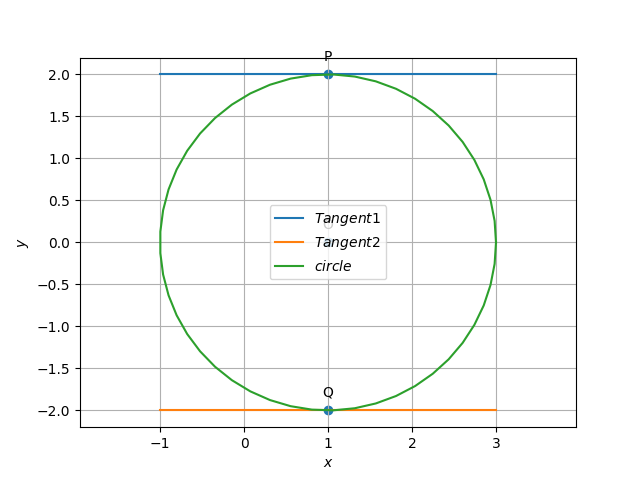
\includegraphics[width=\columnwidth]{./figs/circex/CircTangent.eps}
\caption{Tangents are parallel to the $x$-axis. }
\label{fig:CircTangent}	
\end{figure}

\end{enumerate}
}
\caption{}
\label{fig:8.5.16_circle_latex}	
\end{figure}
%
%
%\renewcommand{\thefigure}{\theenumi}
%
\item {\em Construction: }In Fig. \ref{fig:8.5.16_circle_latex} the known parameters are
%\label{}
\\
%
%\solution From the given information, 
%$\triangle ABC$ are 
\begin{align}
\vec{O} &= \myvec{0\\0} ,
\\
\vec{A} &= \myvec{r\\0} ,
\label{eq:8.5.16_constr_a}
\\
 \vec{B} &= \myvec{-r\\0} 
\label{eq:8.5.16_constr_b}
\\
\vec{C}&= r\myvec{\cos\theta\\\sin\theta}
\label{eq:8.5.16_constr_cgen}
\end{align}
%
Let 
\begin{align}
\vec{D} & = r\myvec{\cos\theta_1\\\sin\theta_1} 
\label{eq:8.5.16_constr_dgen}
\end{align}
From the given information,
\begin{align}
 \norm{\vec{D} - \vec{C}} &= r
\\
\implies \brak{\vec{D} - \vec{C}}^T\brak{\vec{D} - \vec{C}} &= r^2\\
 \label{eq:8.5.16_dist_formula}
\\
\implies  \norm{D} ^2 - 2\vec{D}^T\vec{C} +  \norm{C}^2 &=r^2 
\end{align}
In the above, 
\begin{align}
\because \norm{D} &= \norm{\vec{C}} = r,
\\
\frac{\vec{D}^T\vec{C}}{\norm{D}\norm{C}}  &= \frac{1}{2}
\\
\implies \cos \brak{\theta_1-\theta} &= 60 \degree
\label{eq:8.5.16_theta_diff}
\end{align}
using the definition of the inner product.  $\because \theta$ is known, we get $\theta_1$ from \eqref{eq:8.5.16_theta_diff}
and $\vec{D}$ from 
\eqref{eq:8.5.16_constr_dgen}. 
%
\subitem Thus,
\begin{align}
BD: \vec{x} &= \vec{B} + \lambda_1 \brak{\vec{B}-\vec{D}}
\\
AC: \vec{x} &= \vec{A} + \lambda_2 \brak{\vec{A}-\vec{C}}
\end{align}
%
which can be used to obtain $\vec{E}$.



General equation of conics is 
\begin{align}
    \vec{x}^T\vec{V}\vec{x}+ 2\vec{u}^T\vec{x}+f = 0
    \label{eq:solutions/1/16/eq:1}
\end{align}
Comparing with the equation given,
\begin{align}
\vec{V}=\myvec{\frac{1}{9} & 0 \\ 0 & \frac{1}{16}}\\
\vec{u}=\vec{0}\\
f=-1\\
\mydet{\vec{v}}=\mydet{\myvec{\frac{1}{9} & 0 \\ 0 & \frac{1}{16}}}>0
\end{align}
$\because \abs{\vec{V}}>0$, the given equation is of ellipse.\\
a)The tangents are parallel to the x-axis, hence, their direction and normal vectors, $\vec{m_1}$ and $\vec{n_1}$ are respectively,
\begin{align}
\vec{m_1}=\myvec{1\\0}\\
\vec{n_1}=\myvec{0\\1}
\end{align}
For an ellipse, given the normal vector $\vec{n}$, the tangent points of contact to the ellipse are given by
\begin{align}
    \vec{q}=\vec{V}^{-1}(\kappa \vec{n}-\vec{u})
    \label{eq:solutions/1/16/eq:2}
    =\vec{V}^{-1}\kappa \vec{n}
\end{align}
where
\begin{align}
    \kappa=\pm \sqrt{\frac{\vec{u^T}\vec{V}^{-1}\vec{u}-f}{\vec{n^T}\vec{V}^{-1}\vec{n}}}
    \label{eq:solutions/1/16/eq:2.0.9}\\
   =\pm \sqrt{\frac{-f}{\vec{n^T}\vec{V}^{-1}\vec{n}}}\\
    \vec{V}^{-1}=\myvec{9 & 0 \\ 0 & 16}\\
    \kappa_1=\pm \sqrt{\frac{-(-1)}{\myvec{0 & 1}\myvec{9 & 0 \\ 0 & 16} \myvec{0\\1}}}\\
 \implies \kappa_1=\pm \sqrt{\frac{1}{16}}\\
    \implies \kappa_1=\pm \frac{1}{4}      
\end{align}
From \eqref{eq:solutions/1/16/eq:2} , the point of contact $\vec{q_i}$ are,
\begin{align}
    \vec{q_1}=\myvec{9 & 0 \\ 0 & 16}\frac{1}{4}\myvec{0\\1}\\
    =\myvec{9 & 0 \\ 0 & 16}\myvec{0\\\frac{1}{4}}\\
    =\myvec{0\\4}\\
    \vec{q_2}=\myvec{9 & 0 \\ 0 & 16}\left(-\frac{1}{4}\right)\ \myvec{0\\1}\\
    =\myvec{9 & 0 \\ 0 & 16}\myvec{0\\-\frac{1}{4}}\\
    =\myvec{0\\-4}
\end{align}
b) The tangents are parallel to the y-axis, hence, their direction and normal vectors, $\vec{m_2}$ and $\vec{n_2}$ are respectively,
\begin{align}
\vec{m_2}=\myvec{0\\1}\\
\vec{n_2}=\myvec{1\\0}
\end{align}
Using equation \eqref{eq:solutions/1/16/eq:2.0.9}, the values of $\kappa$ for this case are
\begin{align}
     \kappa_2=\pm \sqrt{\frac{-(-1)}{\myvec{1 & 0}\myvec{9 & 0 \\ 0 & 16} \myvec{1\\0}}}\\
 \implies \kappa_2=\pm \sqrt{\frac{1}{9}}\\
    \implies \kappa_2=\pm \frac{1}{3} 
\end{align}
and from \eqref{eq:solutions/1/16/eq:2} , the point of contact $\vec{q_i}$ are,
\begin{align}
\vec{q_3}=\myvec{9 & 0 \\ 0 & 16}\frac{1}{3}\myvec{1\\0}\\
    =\myvec{9 & 0 \\ 0 & 16}\myvec{\frac{1}{3}\\0}\\
    =\myvec{3\\0}\\
\vec{q_4}=\myvec{9 & 0 \\ 0 & 16}\left(-\frac{1}{3}\right)\ \myvec{1\\0}\\
    =\myvec{9 & 0 \\ 0 & 16}\myvec{-\frac{1}{3}\\0}\\
    =\myvec{-3\\0}
\end{align}
 \begin{figure}[h!]
	\centering
	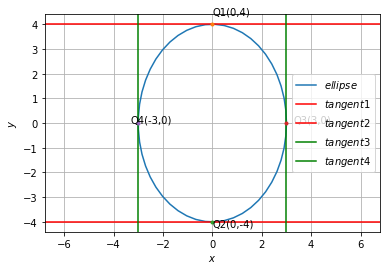
\includegraphics[width=\columnwidth]{./solutions/conics/1/16/ellipse.png}
	\caption{Figure depicting point of contact of tangents of ellipse parallel to x-axis and y-axis}
	\label{eq:solutions/1/16/fig1}
\end{figure}

\end{enumerate}

\item $ABCD$ is a cyclic quadrilateral in which $AC$ and $BD$ are its diagonals. If $\angle DBC = 55\degree$ and $\angle BAC = 45\degree$, find $\angle BCD$
\item Two circles intersect at two points $A and B$. $AD$ and $AC$ are diameters to the two circles. Prove that $B$ lies on the line segment $DC$.
\item Prove that the quadrilateral formed (if possible) by the internal angle bisectors of any quadrilateral is cyclic.
\begin{enumerate}

%\renewcommand{\thefigure}{\theenumi.\arabic{figure}}
\begin{figure}[!ht]
\centering
\resizebox{\columnwidth}{!}{\renewcommand{\theequation}{\theenumi}
\begin{enumerate}[label=\thesection.\arabic*.,ref=\thesection.\theenumi]
\numberwithin{equation}{enumi}
\item  Find the centre and radius of the circle 
\begin{align}
x^2+y^2+8x+10y-8 = 0
\label{eq:circ_basic}
\end{align}
\solution
\eqref{eq:circ_basic} can be expressed as 
\begin{align}
\vec{x}^T\vec{x}+ 2\myvec{4 & 5}\vec{x} -8 = 0
\end{align}
which is of the form \eqref{eq:conic_quad_form} with
\begin{align}
\label{eq:circ_basic_uf}
\vec{u} = \myvec{4\\5}, f = -8
\end{align}
From  Table \ref{table:conics}, the center and radius are given by 
\begin{align}
\vec{c} = -\vec{u} = \myvec{-4\\-5},
r = \sqrt{\norm{u}^2-f} = 7
\end{align}
\item Find the equation of a circle which passes through the points $\vec{P} = \myvec{2\\-2}$ and $\vec{Q} = \myvec{3\\4}$ and whose centre lies on the line  
%\cite{eleven}
\begin{align}
\label{eq:circ_ex1_line}
\myvec{1 & 1} \vec{x} = 2
\end{align}
\solution From \eqref{eq:conic_quad_form} and Table \ref{table:conics}, the equation of a circle can be expressed as
\begin{align}
\label{eq:circ_conic}
\vec{x}^T\vec{x}-2\vec{c}^T\vec{x}+f = 0
\end{align}
where $\vec{c}$ is the centre.
Substituting the given points in 
\eqref{eq:circ_conic} and using 
\eqref{eq:circ_ex1_line}, the following equations are obtained
\begin{align}
2\myvec{2 & -2}\vec{c} -  f &= 8
\\
2\myvec{3 & 4}\vec{c} -  f &= 25
\\
\myvec{1 & 1}\vec{c}  &= 2
\end{align}
which can be expressed as the matrix equation
\begin{align}
\myvec{
1 & 1 & 0
\\
4 & -4 & -1 
\\ 
6 & 8 & -1  
}
\myvec{\vec{c}\\f} = \myvec{2\\8\\25}
\end{align}
Row reducing the augmented matrix
\begin{align}
\myvec{
1 & 1 & 0 & 2
\\
4 & -4 & -1 & 8
\\ 
6 & 8 & -1  & 25
}
\\
\xleftrightarrow[R_3 \leftarrow R_3 -6R_1]{R_2 \leftarrow -R_2+4R_1}
\myvec{
1 & 1 & 0 & 2
\\
0 & 8 & 1 & 0
\\ 
0 & 2 & -1  & 13
}
\\
\xleftrightarrow[R_3 \leftarrow -\frac{4R_3 -R_2}{2}]{R_1 \leftarrow 8R_1-R_3}
\myvec{
8 & 0 & -1 & 16
\\
0 & 8 & 1 & 0
\\ 
0 & 0 & 5  & -52
}
\\
\xleftrightarrow[R_2 \leftarrow \frac{5R_2 -R_3}{4}]{R_1 \leftarrow \frac{5R_1+R_3}{4}}
\myvec{
10 & 0 & 0 & 7
\\
0 & 10 & 0 & 13
\\ 
0 & 0 & 5  & -52
}
\end{align}
Thus, 
\begin{align}
\vec{c} &= \frac{1}{10}\myvec{7\\13}
\\
f &=-\frac{52}{5}
\end{align}
which give the desired equation of the circle.
From Table \ref{table:conics},
%
\begin{align}
 r =  \sqrt{\norm{\vec{c}}^2-f} = \frac{1}{10}\sqrt{1258}
\end{align}
Fig. \ref{fig:CircOr}	verifies the above results.

\begin{figure}[!ht]
\centering
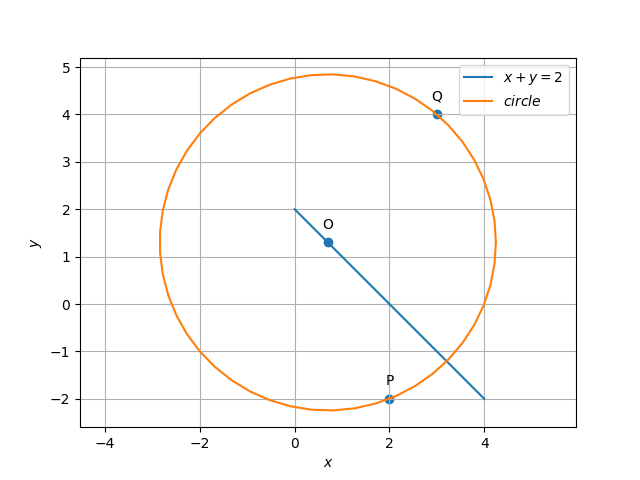
\includegraphics[width=\columnwidth]{./figs/circex/CircOr.eps}
\caption{Circle passing through $\myvec{2\\-2},\myvec{3\\4}$. Center is on line $\myvec{1 & 1}\vec{x}=2$. }
\label{fig:CircOr}	
\end{figure}

\item 
Find the points on the curve  
%\cite{twelve_one}
\begin{align}
x^2+y^2-2x-3 = 0
\label{eq:circle_tangent_prob}
\end{align}
at which the tangents are parallel to the $x$-axis.
\\
\solution \eqref{eq:circle_tangent_prob} can be expressed as
\begin{align}
\vec{x}^T\vec{x}+\myvec{-2 & 0}\vec{x}-3 &= 0
\label{eq:circle_tangent_prob_vec}
\\
\implies \vec{V} = \vec{I}, \vec{u} = \myvec{-1 \\ 0}, f = -3
\label{eq:circle_tangent_prob_uf}
\end{align}
From Table \ref{table:conics}, the centre and radius are
\begin{align}
\vec{c} = -\vec{u} = \myvec{-1 \\ 0}, r =\sqrt{\norm{\vec{u}}^2-f} = 2
\end{align}
$\because$ the tangents are parallel to the $x$-axis, their direction and normal vectors are respectively,
\begin{align}
\vec{m} = \myvec{1\\0},
\vec{n} = \myvec{0\\1}.
\end{align}
From Table \ref{table:conics},
\begin{align}
\kappa = \pm \sqrt{\frac{\vec{u}^T\vec{u}-f}{\vec{n}^T\vec{n}}} = \pm \sqrt{\frac{4}{1}} = \pm 2
\end{align}
and the desired points of contact are 
\begin{align}
\vec{q}_1, \vec{q}_2 = \myvec{1\\0}\pm 2\myvec{0\\1} =  
\myvec{1 \\  2},
\myvec{1 \\  -2}
\end{align}
%
Fig. \ref{fig:CircOr}	verifies the above results.
\begin{figure}[!ht]
\centering
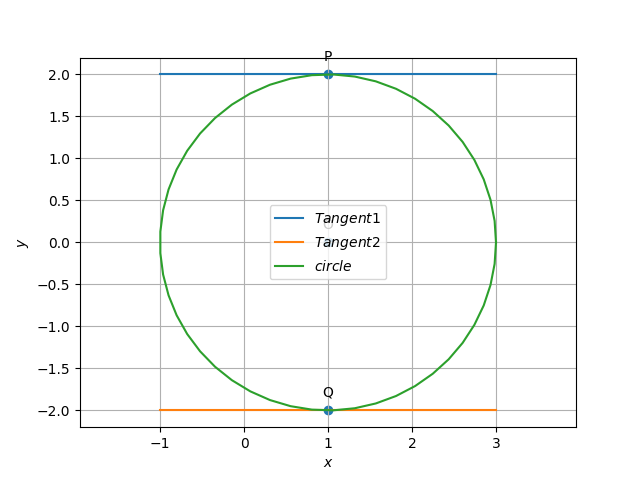
\includegraphics[width=\columnwidth]{./figs/circex/CircTangent.eps}
\caption{Tangents are parallel to the $x$-axis. }
\label{fig:CircTangent}	
\end{figure}

\end{enumerate}
}
\caption{}
\label{fig:8.5.16_circle_latex}	
\end{figure}
%
%
%\renewcommand{\thefigure}{\theenumi}
%
\item {\em Construction: }In Fig. \ref{fig:8.5.16_circle_latex} the known parameters are
%\label{}
\\
%
%\solution From the given information, 
%$\triangle ABC$ are 
\begin{align}
\vec{O} &= \myvec{0\\0} ,
\\
\vec{A} &= \myvec{r\\0} ,
\label{eq:8.5.16_constr_a}
\\
 \vec{B} &= \myvec{-r\\0} 
\label{eq:8.5.16_constr_b}
\\
\vec{C}&= r\myvec{\cos\theta\\\sin\theta}
\label{eq:8.5.16_constr_cgen}
\end{align}
%
Let 
\begin{align}
\vec{D} & = r\myvec{\cos\theta_1\\\sin\theta_1} 
\label{eq:8.5.16_constr_dgen}
\end{align}
From the given information,
\begin{align}
 \norm{\vec{D} - \vec{C}} &= r
\\
\implies \brak{\vec{D} - \vec{C}}^T\brak{\vec{D} - \vec{C}} &= r^2\\
 \label{eq:8.5.16_dist_formula}
\\
\implies  \norm{D} ^2 - 2\vec{D}^T\vec{C} +  \norm{C}^2 &=r^2 
\end{align}
In the above, 
\begin{align}
\because \norm{D} &= \norm{\vec{C}} = r,
\\
\frac{\vec{D}^T\vec{C}}{\norm{D}\norm{C}}  &= \frac{1}{2}
\\
\implies \cos \brak{\theta_1-\theta} &= 60 \degree
\label{eq:8.5.16_theta_diff}
\end{align}
using the definition of the inner product.  $\because \theta$ is known, we get $\theta_1$ from \eqref{eq:8.5.16_theta_diff}
and $\vec{D}$ from 
\eqref{eq:8.5.16_constr_dgen}. 
%
\subitem Thus,
\begin{align}
BD: \vec{x} &= \vec{B} + \lambda_1 \brak{\vec{B}-\vec{D}}
\\
AC: \vec{x} &= \vec{A} + \lambda_2 \brak{\vec{A}-\vec{C}}
\end{align}
%
which can be used to obtain $\vec{E}$.



General equation of conics is 
\begin{align}
    \vec{x}^T\vec{V}\vec{x}+ 2\vec{u}^T\vec{x}+f = 0
    \label{eq:solutions/1/16/eq:1}
\end{align}
Comparing with the equation given,
\begin{align}
\vec{V}=\myvec{\frac{1}{9} & 0 \\ 0 & \frac{1}{16}}\\
\vec{u}=\vec{0}\\
f=-1\\
\mydet{\vec{v}}=\mydet{\myvec{\frac{1}{9} & 0 \\ 0 & \frac{1}{16}}}>0
\end{align}
$\because \abs{\vec{V}}>0$, the given equation is of ellipse.\\
a)The tangents are parallel to the x-axis, hence, their direction and normal vectors, $\vec{m_1}$ and $\vec{n_1}$ are respectively,
\begin{align}
\vec{m_1}=\myvec{1\\0}\\
\vec{n_1}=\myvec{0\\1}
\end{align}
For an ellipse, given the normal vector $\vec{n}$, the tangent points of contact to the ellipse are given by
\begin{align}
    \vec{q}=\vec{V}^{-1}(\kappa \vec{n}-\vec{u})
    \label{eq:solutions/1/16/eq:2}
    =\vec{V}^{-1}\kappa \vec{n}
\end{align}
where
\begin{align}
    \kappa=\pm \sqrt{\frac{\vec{u^T}\vec{V}^{-1}\vec{u}-f}{\vec{n^T}\vec{V}^{-1}\vec{n}}}
    \label{eq:solutions/1/16/eq:2.0.9}\\
   =\pm \sqrt{\frac{-f}{\vec{n^T}\vec{V}^{-1}\vec{n}}}\\
    \vec{V}^{-1}=\myvec{9 & 0 \\ 0 & 16}\\
    \kappa_1=\pm \sqrt{\frac{-(-1)}{\myvec{0 & 1}\myvec{9 & 0 \\ 0 & 16} \myvec{0\\1}}}\\
 \implies \kappa_1=\pm \sqrt{\frac{1}{16}}\\
    \implies \kappa_1=\pm \frac{1}{4}      
\end{align}
From \eqref{eq:solutions/1/16/eq:2} , the point of contact $\vec{q_i}$ are,
\begin{align}
    \vec{q_1}=\myvec{9 & 0 \\ 0 & 16}\frac{1}{4}\myvec{0\\1}\\
    =\myvec{9 & 0 \\ 0 & 16}\myvec{0\\\frac{1}{4}}\\
    =\myvec{0\\4}\\
    \vec{q_2}=\myvec{9 & 0 \\ 0 & 16}\left(-\frac{1}{4}\right)\ \myvec{0\\1}\\
    =\myvec{9 & 0 \\ 0 & 16}\myvec{0\\-\frac{1}{4}}\\
    =\myvec{0\\-4}
\end{align}
b) The tangents are parallel to the y-axis, hence, their direction and normal vectors, $\vec{m_2}$ and $\vec{n_2}$ are respectively,
\begin{align}
\vec{m_2}=\myvec{0\\1}\\
\vec{n_2}=\myvec{1\\0}
\end{align}
Using equation \eqref{eq:solutions/1/16/eq:2.0.9}, the values of $\kappa$ for this case are
\begin{align}
     \kappa_2=\pm \sqrt{\frac{-(-1)}{\myvec{1 & 0}\myvec{9 & 0 \\ 0 & 16} \myvec{1\\0}}}\\
 \implies \kappa_2=\pm \sqrt{\frac{1}{9}}\\
    \implies \kappa_2=\pm \frac{1}{3} 
\end{align}
and from \eqref{eq:solutions/1/16/eq:2} , the point of contact $\vec{q_i}$ are,
\begin{align}
\vec{q_3}=\myvec{9 & 0 \\ 0 & 16}\frac{1}{3}\myvec{1\\0}\\
    =\myvec{9 & 0 \\ 0 & 16}\myvec{\frac{1}{3}\\0}\\
    =\myvec{3\\0}\\
\vec{q_4}=\myvec{9 & 0 \\ 0 & 16}\left(-\frac{1}{3}\right)\ \myvec{1\\0}\\
    =\myvec{9 & 0 \\ 0 & 16}\myvec{-\frac{1}{3}\\0}\\
    =\myvec{-3\\0}
\end{align}
 \begin{figure}[h!]
	\centering
	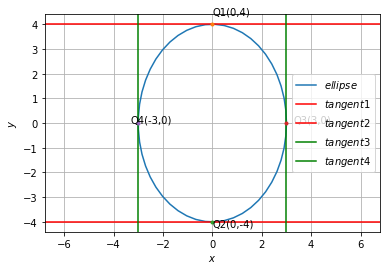
\includegraphics[width=\columnwidth]{./solutions/conics/1/16/ellipse.png}
	\caption{Figure depicting point of contact of tangents of ellipse parallel to x-axis and y-axis}
	\label{eq:solutions/1/16/fig1}
\end{figure}

\end{enumerate}

\item  Equal chords of a circle (or of congruent circles) subtend equal angles at the centre. 
\item  If the angles subtended by two chords of a circle (or of congruent circles) at the centre (corresponding centres) are equal, the chords are equal.
\item  The perpendicular from the centre of a circle to a chord bisects the chord. 
\item  The line drawn through the centre of a circle to bisect a chord is perpendicular to the chord.
\item  There is one and only one circle passing through three non-collinear points. 
\item  Equal chords of a circle (or of congruent circles) are equidistant from the centre (or corresponding centres).
\item Chords equidistant from the centre (or corresponding centres) of a circle (or of congruent circles) are equal.
\item  If two arcs of a circle are congruent, then their corresponding chords are equal and conversely if two chords of a circle are equal, then their corresponding arcs (minor, major) are congruent.
\item Congruent arcs of a circle subtend equal angles at the centre. 
\item  The angle subtended by an arc at the centre is double the angle subtended by it at any point on the remaining part of the circle.
\item Angles in the same segment of a circle are equal. \item  Angle in a semicircle is a right angle. 
\item  If a line segment joining two points subtends equal angles at two other points lying on the same side of the line containing the line segment, the four points lie on a circle. 
\item  The sum of either pair of opposite angles of a cyclic quadrilateral is 180$\degree$.
\item  If sum of a pair of opposite angles of a quadrilateral is 180$\degree$, the quadrilateral is cyclic.
%
\item AB is a diameter of the circle, $CD$ is a chord equal to the radius of the circle. $AC$ and $BD$ when extended intersect at a point $E$. Prove that $\angle AEB = 60\degree$.
\item Two circles intersect at two points $A$ and $B$. $AD$ and $AC$ are diameters to the two circles. Prove that $B$ lies on the line segment $DC$.
\item Prove that the quadrilateral formed (if possible) by the internal angle bisectors of any quadrilateral is cyclic.
\item  If two equal chords of a circle intersect within the circle, prove that the segments of one chord are equal to corresponding segments of the other chord.
\item If two equal chords of a circle intersect within the circle, prove that the line joining the point of intersection to the centre makes equal angles with the chords.
\begin{enumerate}

%\renewcommand{\thefigure}{\theenumi.\arabic{figure}}
\begin{figure}[!ht]
\centering
\resizebox{\columnwidth}{!}{\renewcommand{\theequation}{\theenumi}
\begin{enumerate}[label=\thesection.\arabic*.,ref=\thesection.\theenumi]
\numberwithin{equation}{enumi}
\item  Find the centre and radius of the circle 
\begin{align}
x^2+y^2+8x+10y-8 = 0
\label{eq:circ_basic}
\end{align}
\solution
\eqref{eq:circ_basic} can be expressed as 
\begin{align}
\vec{x}^T\vec{x}+ 2\myvec{4 & 5}\vec{x} -8 = 0
\end{align}
which is of the form \eqref{eq:conic_quad_form} with
\begin{align}
\label{eq:circ_basic_uf}
\vec{u} = \myvec{4\\5}, f = -8
\end{align}
From  Table \ref{table:conics}, the center and radius are given by 
\begin{align}
\vec{c} = -\vec{u} = \myvec{-4\\-5},
r = \sqrt{\norm{u}^2-f} = 7
\end{align}
\item Find the equation of a circle which passes through the points $\vec{P} = \myvec{2\\-2}$ and $\vec{Q} = \myvec{3\\4}$ and whose centre lies on the line  
%\cite{eleven}
\begin{align}
\label{eq:circ_ex1_line}
\myvec{1 & 1} \vec{x} = 2
\end{align}
\solution From \eqref{eq:conic_quad_form} and Table \ref{table:conics}, the equation of a circle can be expressed as
\begin{align}
\label{eq:circ_conic}
\vec{x}^T\vec{x}-2\vec{c}^T\vec{x}+f = 0
\end{align}
where $\vec{c}$ is the centre.
Substituting the given points in 
\eqref{eq:circ_conic} and using 
\eqref{eq:circ_ex1_line}, the following equations are obtained
\begin{align}
2\myvec{2 & -2}\vec{c} -  f &= 8
\\
2\myvec{3 & 4}\vec{c} -  f &= 25
\\
\myvec{1 & 1}\vec{c}  &= 2
\end{align}
which can be expressed as the matrix equation
\begin{align}
\myvec{
1 & 1 & 0
\\
4 & -4 & -1 
\\ 
6 & 8 & -1  
}
\myvec{\vec{c}\\f} = \myvec{2\\8\\25}
\end{align}
Row reducing the augmented matrix
\begin{align}
\myvec{
1 & 1 & 0 & 2
\\
4 & -4 & -1 & 8
\\ 
6 & 8 & -1  & 25
}
\\
\xleftrightarrow[R_3 \leftarrow R_3 -6R_1]{R_2 \leftarrow -R_2+4R_1}
\myvec{
1 & 1 & 0 & 2
\\
0 & 8 & 1 & 0
\\ 
0 & 2 & -1  & 13
}
\\
\xleftrightarrow[R_3 \leftarrow -\frac{4R_3 -R_2}{2}]{R_1 \leftarrow 8R_1-R_3}
\myvec{
8 & 0 & -1 & 16
\\
0 & 8 & 1 & 0
\\ 
0 & 0 & 5  & -52
}
\\
\xleftrightarrow[R_2 \leftarrow \frac{5R_2 -R_3}{4}]{R_1 \leftarrow \frac{5R_1+R_3}{4}}
\myvec{
10 & 0 & 0 & 7
\\
0 & 10 & 0 & 13
\\ 
0 & 0 & 5  & -52
}
\end{align}
Thus, 
\begin{align}
\vec{c} &= \frac{1}{10}\myvec{7\\13}
\\
f &=-\frac{52}{5}
\end{align}
which give the desired equation of the circle.
From Table \ref{table:conics},
%
\begin{align}
 r =  \sqrt{\norm{\vec{c}}^2-f} = \frac{1}{10}\sqrt{1258}
\end{align}
Fig. \ref{fig:CircOr}	verifies the above results.

\begin{figure}[!ht]
\centering
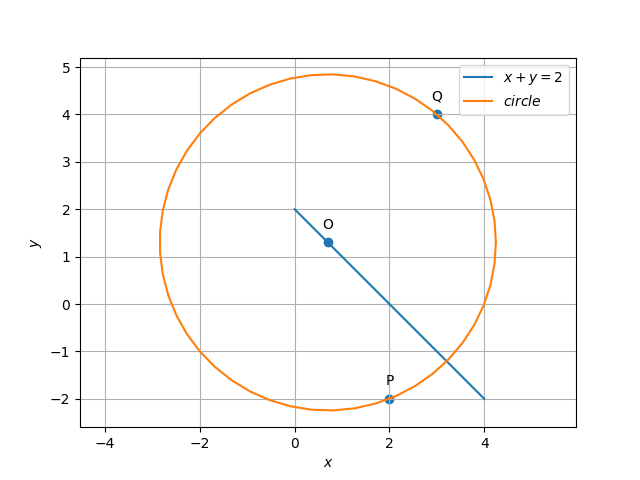
\includegraphics[width=\columnwidth]{./figs/circex/CircOr.eps}
\caption{Circle passing through $\myvec{2\\-2},\myvec{3\\4}$. Center is on line $\myvec{1 & 1}\vec{x}=2$. }
\label{fig:CircOr}	
\end{figure}

\item 
Find the points on the curve  
%\cite{twelve_one}
\begin{align}
x^2+y^2-2x-3 = 0
\label{eq:circle_tangent_prob}
\end{align}
at which the tangents are parallel to the $x$-axis.
\\
\solution \eqref{eq:circle_tangent_prob} can be expressed as
\begin{align}
\vec{x}^T\vec{x}+\myvec{-2 & 0}\vec{x}-3 &= 0
\label{eq:circle_tangent_prob_vec}
\\
\implies \vec{V} = \vec{I}, \vec{u} = \myvec{-1 \\ 0}, f = -3
\label{eq:circle_tangent_prob_uf}
\end{align}
From Table \ref{table:conics}, the centre and radius are
\begin{align}
\vec{c} = -\vec{u} = \myvec{-1 \\ 0}, r =\sqrt{\norm{\vec{u}}^2-f} = 2
\end{align}
$\because$ the tangents are parallel to the $x$-axis, their direction and normal vectors are respectively,
\begin{align}
\vec{m} = \myvec{1\\0},
\vec{n} = \myvec{0\\1}.
\end{align}
From Table \ref{table:conics},
\begin{align}
\kappa = \pm \sqrt{\frac{\vec{u}^T\vec{u}-f}{\vec{n}^T\vec{n}}} = \pm \sqrt{\frac{4}{1}} = \pm 2
\end{align}
and the desired points of contact are 
\begin{align}
\vec{q}_1, \vec{q}_2 = \myvec{1\\0}\pm 2\myvec{0\\1} =  
\myvec{1 \\  2},
\myvec{1 \\  -2}
\end{align}
%
Fig. \ref{fig:CircOr}	verifies the above results.
\begin{figure}[!ht]
\centering
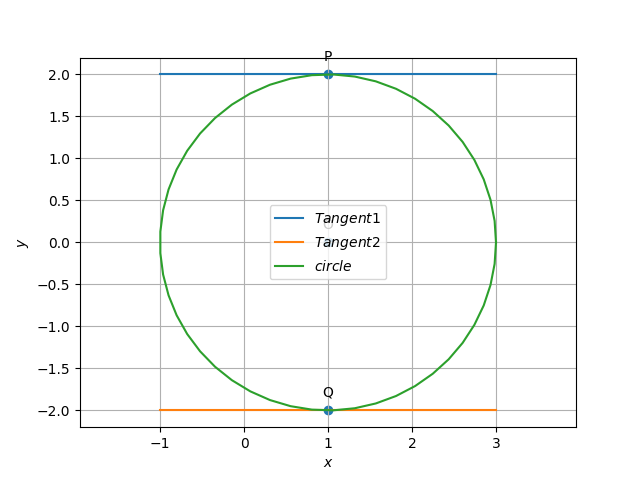
\includegraphics[width=\columnwidth]{./figs/circex/CircTangent.eps}
\caption{Tangents are parallel to the $x$-axis. }
\label{fig:CircTangent}	
\end{figure}

\end{enumerate}
}
\caption{}
\label{fig:8.5.16_circle_latex}	
\end{figure}
%
%
%\renewcommand{\thefigure}{\theenumi}
%
\item {\em Construction: }In Fig. \ref{fig:8.5.16_circle_latex} the known parameters are
%\label{}
\\
%
%\solution From the given information, 
%$\triangle ABC$ are 
\begin{align}
\vec{O} &= \myvec{0\\0} ,
\\
\vec{A} &= \myvec{r\\0} ,
\label{eq:8.5.16_constr_a}
\\
 \vec{B} &= \myvec{-r\\0} 
\label{eq:8.5.16_constr_b}
\\
\vec{C}&= r\myvec{\cos\theta\\\sin\theta}
\label{eq:8.5.16_constr_cgen}
\end{align}
%
Let 
\begin{align}
\vec{D} & = r\myvec{\cos\theta_1\\\sin\theta_1} 
\label{eq:8.5.16_constr_dgen}
\end{align}
From the given information,
\begin{align}
 \norm{\vec{D} - \vec{C}} &= r
\\
\implies \brak{\vec{D} - \vec{C}}^T\brak{\vec{D} - \vec{C}} &= r^2\\
 \label{eq:8.5.16_dist_formula}
\\
\implies  \norm{D} ^2 - 2\vec{D}^T\vec{C} +  \norm{C}^2 &=r^2 
\end{align}
In the above, 
\begin{align}
\because \norm{D} &= \norm{\vec{C}} = r,
\\
\frac{\vec{D}^T\vec{C}}{\norm{D}\norm{C}}  &= \frac{1}{2}
\\
\implies \cos \brak{\theta_1-\theta} &= 60 \degree
\label{eq:8.5.16_theta_diff}
\end{align}
using the definition of the inner product.  $\because \theta$ is known, we get $\theta_1$ from \eqref{eq:8.5.16_theta_diff}
and $\vec{D}$ from 
\eqref{eq:8.5.16_constr_dgen}. 
%
\subitem Thus,
\begin{align}
BD: \vec{x} &= \vec{B} + \lambda_1 \brak{\vec{B}-\vec{D}}
\\
AC: \vec{x} &= \vec{A} + \lambda_2 \brak{\vec{A}-\vec{C}}
\end{align}
%
which can be used to obtain $\vec{E}$.



General equation of conics is 
\begin{align}
    \vec{x}^T\vec{V}\vec{x}+ 2\vec{u}^T\vec{x}+f = 0
    \label{eq:solutions/1/16/eq:1}
\end{align}
Comparing with the equation given,
\begin{align}
\vec{V}=\myvec{\frac{1}{9} & 0 \\ 0 & \frac{1}{16}}\\
\vec{u}=\vec{0}\\
f=-1\\
\mydet{\vec{v}}=\mydet{\myvec{\frac{1}{9} & 0 \\ 0 & \frac{1}{16}}}>0
\end{align}
$\because \abs{\vec{V}}>0$, the given equation is of ellipse.\\
a)The tangents are parallel to the x-axis, hence, their direction and normal vectors, $\vec{m_1}$ and $\vec{n_1}$ are respectively,
\begin{align}
\vec{m_1}=\myvec{1\\0}\\
\vec{n_1}=\myvec{0\\1}
\end{align}
For an ellipse, given the normal vector $\vec{n}$, the tangent points of contact to the ellipse are given by
\begin{align}
    \vec{q}=\vec{V}^{-1}(\kappa \vec{n}-\vec{u})
    \label{eq:solutions/1/16/eq:2}
    =\vec{V}^{-1}\kappa \vec{n}
\end{align}
where
\begin{align}
    \kappa=\pm \sqrt{\frac{\vec{u^T}\vec{V}^{-1}\vec{u}-f}{\vec{n^T}\vec{V}^{-1}\vec{n}}}
    \label{eq:solutions/1/16/eq:2.0.9}\\
   =\pm \sqrt{\frac{-f}{\vec{n^T}\vec{V}^{-1}\vec{n}}}\\
    \vec{V}^{-1}=\myvec{9 & 0 \\ 0 & 16}\\
    \kappa_1=\pm \sqrt{\frac{-(-1)}{\myvec{0 & 1}\myvec{9 & 0 \\ 0 & 16} \myvec{0\\1}}}\\
 \implies \kappa_1=\pm \sqrt{\frac{1}{16}}\\
    \implies \kappa_1=\pm \frac{1}{4}      
\end{align}
From \eqref{eq:solutions/1/16/eq:2} , the point of contact $\vec{q_i}$ are,
\begin{align}
    \vec{q_1}=\myvec{9 & 0 \\ 0 & 16}\frac{1}{4}\myvec{0\\1}\\
    =\myvec{9 & 0 \\ 0 & 16}\myvec{0\\\frac{1}{4}}\\
    =\myvec{0\\4}\\
    \vec{q_2}=\myvec{9 & 0 \\ 0 & 16}\left(-\frac{1}{4}\right)\ \myvec{0\\1}\\
    =\myvec{9 & 0 \\ 0 & 16}\myvec{0\\-\frac{1}{4}}\\
    =\myvec{0\\-4}
\end{align}
b) The tangents are parallel to the y-axis, hence, their direction and normal vectors, $\vec{m_2}$ and $\vec{n_2}$ are respectively,
\begin{align}
\vec{m_2}=\myvec{0\\1}\\
\vec{n_2}=\myvec{1\\0}
\end{align}
Using equation \eqref{eq:solutions/1/16/eq:2.0.9}, the values of $\kappa$ for this case are
\begin{align}
     \kappa_2=\pm \sqrt{\frac{-(-1)}{\myvec{1 & 0}\myvec{9 & 0 \\ 0 & 16} \myvec{1\\0}}}\\
 \implies \kappa_2=\pm \sqrt{\frac{1}{9}}\\
    \implies \kappa_2=\pm \frac{1}{3} 
\end{align}
and from \eqref{eq:solutions/1/16/eq:2} , the point of contact $\vec{q_i}$ are,
\begin{align}
\vec{q_3}=\myvec{9 & 0 \\ 0 & 16}\frac{1}{3}\myvec{1\\0}\\
    =\myvec{9 & 0 \\ 0 & 16}\myvec{\frac{1}{3}\\0}\\
    =\myvec{3\\0}\\
\vec{q_4}=\myvec{9 & 0 \\ 0 & 16}\left(-\frac{1}{3}\right)\ \myvec{1\\0}\\
    =\myvec{9 & 0 \\ 0 & 16}\myvec{-\frac{1}{3}\\0}\\
    =\myvec{-3\\0}
\end{align}
 \begin{figure}[h!]
	\centering
	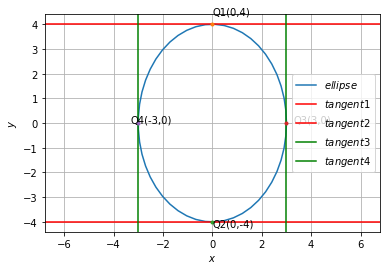
\includegraphics[width=\columnwidth]{./solutions/conics/1/16/ellipse.png}
	\caption{Figure depicting point of contact of tangents of ellipse parallel to x-axis and y-axis}
	\label{eq:solutions/1/16/fig1}
\end{figure}

\end{enumerate}

\item If a line intersects two concentric circles (circles with the same centre) with centre O at A, B, C and D, prove that AB = CD.
\begin{enumerate}

%\renewcommand{\thefigure}{\theenumi.\arabic{figure}}
\begin{figure}[!ht]
\centering
\resizebox{\columnwidth}{!}{\renewcommand{\theequation}{\theenumi}
\begin{enumerate}[label=\thesection.\arabic*.,ref=\thesection.\theenumi]
\numberwithin{equation}{enumi}
\item  Find the centre and radius of the circle 
\begin{align}
x^2+y^2+8x+10y-8 = 0
\label{eq:circ_basic}
\end{align}
\solution
\eqref{eq:circ_basic} can be expressed as 
\begin{align}
\vec{x}^T\vec{x}+ 2\myvec{4 & 5}\vec{x} -8 = 0
\end{align}
which is of the form \eqref{eq:conic_quad_form} with
\begin{align}
\label{eq:circ_basic_uf}
\vec{u} = \myvec{4\\5}, f = -8
\end{align}
From  Table \ref{table:conics}, the center and radius are given by 
\begin{align}
\vec{c} = -\vec{u} = \myvec{-4\\-5},
r = \sqrt{\norm{u}^2-f} = 7
\end{align}
\item Find the equation of a circle which passes through the points $\vec{P} = \myvec{2\\-2}$ and $\vec{Q} = \myvec{3\\4}$ and whose centre lies on the line  
%\cite{eleven}
\begin{align}
\label{eq:circ_ex1_line}
\myvec{1 & 1} \vec{x} = 2
\end{align}
\solution From \eqref{eq:conic_quad_form} and Table \ref{table:conics}, the equation of a circle can be expressed as
\begin{align}
\label{eq:circ_conic}
\vec{x}^T\vec{x}-2\vec{c}^T\vec{x}+f = 0
\end{align}
where $\vec{c}$ is the centre.
Substituting the given points in 
\eqref{eq:circ_conic} and using 
\eqref{eq:circ_ex1_line}, the following equations are obtained
\begin{align}
2\myvec{2 & -2}\vec{c} -  f &= 8
\\
2\myvec{3 & 4}\vec{c} -  f &= 25
\\
\myvec{1 & 1}\vec{c}  &= 2
\end{align}
which can be expressed as the matrix equation
\begin{align}
\myvec{
1 & 1 & 0
\\
4 & -4 & -1 
\\ 
6 & 8 & -1  
}
\myvec{\vec{c}\\f} = \myvec{2\\8\\25}
\end{align}
Row reducing the augmented matrix
\begin{align}
\myvec{
1 & 1 & 0 & 2
\\
4 & -4 & -1 & 8
\\ 
6 & 8 & -1  & 25
}
\\
\xleftrightarrow[R_3 \leftarrow R_3 -6R_1]{R_2 \leftarrow -R_2+4R_1}
\myvec{
1 & 1 & 0 & 2
\\
0 & 8 & 1 & 0
\\ 
0 & 2 & -1  & 13
}
\\
\xleftrightarrow[R_3 \leftarrow -\frac{4R_3 -R_2}{2}]{R_1 \leftarrow 8R_1-R_3}
\myvec{
8 & 0 & -1 & 16
\\
0 & 8 & 1 & 0
\\ 
0 & 0 & 5  & -52
}
\\
\xleftrightarrow[R_2 \leftarrow \frac{5R_2 -R_3}{4}]{R_1 \leftarrow \frac{5R_1+R_3}{4}}
\myvec{
10 & 0 & 0 & 7
\\
0 & 10 & 0 & 13
\\ 
0 & 0 & 5  & -52
}
\end{align}
Thus, 
\begin{align}
\vec{c} &= \frac{1}{10}\myvec{7\\13}
\\
f &=-\frac{52}{5}
\end{align}
which give the desired equation of the circle.
From Table \ref{table:conics},
%
\begin{align}
 r =  \sqrt{\norm{\vec{c}}^2-f} = \frac{1}{10}\sqrt{1258}
\end{align}
Fig. \ref{fig:CircOr}	verifies the above results.

\begin{figure}[!ht]
\centering
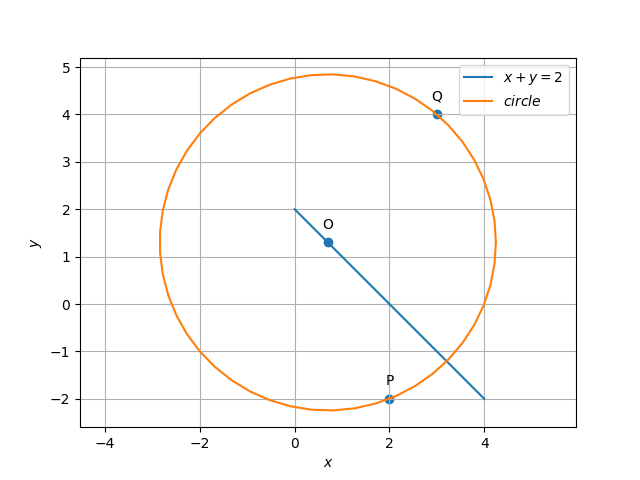
\includegraphics[width=\columnwidth]{./figs/circex/CircOr.eps}
\caption{Circle passing through $\myvec{2\\-2},\myvec{3\\4}$. Center is on line $\myvec{1 & 1}\vec{x}=2$. }
\label{fig:CircOr}	
\end{figure}

\item 
Find the points on the curve  
%\cite{twelve_one}
\begin{align}
x^2+y^2-2x-3 = 0
\label{eq:circle_tangent_prob}
\end{align}
at which the tangents are parallel to the $x$-axis.
\\
\solution \eqref{eq:circle_tangent_prob} can be expressed as
\begin{align}
\vec{x}^T\vec{x}+\myvec{-2 & 0}\vec{x}-3 &= 0
\label{eq:circle_tangent_prob_vec}
\\
\implies \vec{V} = \vec{I}, \vec{u} = \myvec{-1 \\ 0}, f = -3
\label{eq:circle_tangent_prob_uf}
\end{align}
From Table \ref{table:conics}, the centre and radius are
\begin{align}
\vec{c} = -\vec{u} = \myvec{-1 \\ 0}, r =\sqrt{\norm{\vec{u}}^2-f} = 2
\end{align}
$\because$ the tangents are parallel to the $x$-axis, their direction and normal vectors are respectively,
\begin{align}
\vec{m} = \myvec{1\\0},
\vec{n} = \myvec{0\\1}.
\end{align}
From Table \ref{table:conics},
\begin{align}
\kappa = \pm \sqrt{\frac{\vec{u}^T\vec{u}-f}{\vec{n}^T\vec{n}}} = \pm \sqrt{\frac{4}{1}} = \pm 2
\end{align}
and the desired points of contact are 
\begin{align}
\vec{q}_1, \vec{q}_2 = \myvec{1\\0}\pm 2\myvec{0\\1} =  
\myvec{1 \\  2},
\myvec{1 \\  -2}
\end{align}
%
Fig. \ref{fig:CircOr}	verifies the above results.
\begin{figure}[!ht]
\centering
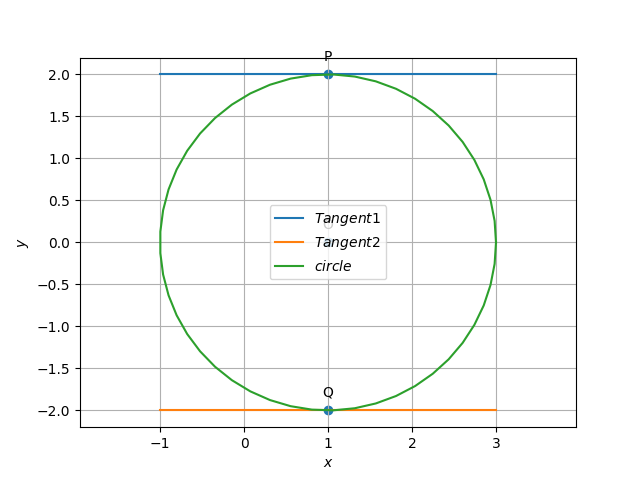
\includegraphics[width=\columnwidth]{./figs/circex/CircTangent.eps}
\caption{Tangents are parallel to the $x$-axis. }
\label{fig:CircTangent}	
\end{figure}

\end{enumerate}
}
\caption{}
\label{fig:8.5.16_circle_latex}	
\end{figure}
%
%
%\renewcommand{\thefigure}{\theenumi}
%
\item {\em Construction: }In Fig. \ref{fig:8.5.16_circle_latex} the known parameters are
%\label{}
\\
%
%\solution From the given information, 
%$\triangle ABC$ are 
\begin{align}
\vec{O} &= \myvec{0\\0} ,
\\
\vec{A} &= \myvec{r\\0} ,
\label{eq:8.5.16_constr_a}
\\
 \vec{B} &= \myvec{-r\\0} 
\label{eq:8.5.16_constr_b}
\\
\vec{C}&= r\myvec{\cos\theta\\\sin\theta}
\label{eq:8.5.16_constr_cgen}
\end{align}
%
Let 
\begin{align}
\vec{D} & = r\myvec{\cos\theta_1\\\sin\theta_1} 
\label{eq:8.5.16_constr_dgen}
\end{align}
From the given information,
\begin{align}
 \norm{\vec{D} - \vec{C}} &= r
\\
\implies \brak{\vec{D} - \vec{C}}^T\brak{\vec{D} - \vec{C}} &= r^2\\
 \label{eq:8.5.16_dist_formula}
\\
\implies  \norm{D} ^2 - 2\vec{D}^T\vec{C} +  \norm{C}^2 &=r^2 
\end{align}
In the above, 
\begin{align}
\because \norm{D} &= \norm{\vec{C}} = r,
\\
\frac{\vec{D}^T\vec{C}}{\norm{D}\norm{C}}  &= \frac{1}{2}
\\
\implies \cos \brak{\theta_1-\theta} &= 60 \degree
\label{eq:8.5.16_theta_diff}
\end{align}
using the definition of the inner product.  $\because \theta$ is known, we get $\theta_1$ from \eqref{eq:8.5.16_theta_diff}
and $\vec{D}$ from 
\eqref{eq:8.5.16_constr_dgen}. 
%
\subitem Thus,
\begin{align}
BD: \vec{x} &= \vec{B} + \lambda_1 \brak{\vec{B}-\vec{D}}
\\
AC: \vec{x} &= \vec{A} + \lambda_2 \brak{\vec{A}-\vec{C}}
\end{align}
%
which can be used to obtain $\vec{E}$.



General equation of conics is 
\begin{align}
    \vec{x}^T\vec{V}\vec{x}+ 2\vec{u}^T\vec{x}+f = 0
    \label{eq:solutions/1/16/eq:1}
\end{align}
Comparing with the equation given,
\begin{align}
\vec{V}=\myvec{\frac{1}{9} & 0 \\ 0 & \frac{1}{16}}\\
\vec{u}=\vec{0}\\
f=-1\\
\mydet{\vec{v}}=\mydet{\myvec{\frac{1}{9} & 0 \\ 0 & \frac{1}{16}}}>0
\end{align}
$\because \abs{\vec{V}}>0$, the given equation is of ellipse.\\
a)The tangents are parallel to the x-axis, hence, their direction and normal vectors, $\vec{m_1}$ and $\vec{n_1}$ are respectively,
\begin{align}
\vec{m_1}=\myvec{1\\0}\\
\vec{n_1}=\myvec{0\\1}
\end{align}
For an ellipse, given the normal vector $\vec{n}$, the tangent points of contact to the ellipse are given by
\begin{align}
    \vec{q}=\vec{V}^{-1}(\kappa \vec{n}-\vec{u})
    \label{eq:solutions/1/16/eq:2}
    =\vec{V}^{-1}\kappa \vec{n}
\end{align}
where
\begin{align}
    \kappa=\pm \sqrt{\frac{\vec{u^T}\vec{V}^{-1}\vec{u}-f}{\vec{n^T}\vec{V}^{-1}\vec{n}}}
    \label{eq:solutions/1/16/eq:2.0.9}\\
   =\pm \sqrt{\frac{-f}{\vec{n^T}\vec{V}^{-1}\vec{n}}}\\
    \vec{V}^{-1}=\myvec{9 & 0 \\ 0 & 16}\\
    \kappa_1=\pm \sqrt{\frac{-(-1)}{\myvec{0 & 1}\myvec{9 & 0 \\ 0 & 16} \myvec{0\\1}}}\\
 \implies \kappa_1=\pm \sqrt{\frac{1}{16}}\\
    \implies \kappa_1=\pm \frac{1}{4}      
\end{align}
From \eqref{eq:solutions/1/16/eq:2} , the point of contact $\vec{q_i}$ are,
\begin{align}
    \vec{q_1}=\myvec{9 & 0 \\ 0 & 16}\frac{1}{4}\myvec{0\\1}\\
    =\myvec{9 & 0 \\ 0 & 16}\myvec{0\\\frac{1}{4}}\\
    =\myvec{0\\4}\\
    \vec{q_2}=\myvec{9 & 0 \\ 0 & 16}\left(-\frac{1}{4}\right)\ \myvec{0\\1}\\
    =\myvec{9 & 0 \\ 0 & 16}\myvec{0\\-\frac{1}{4}}\\
    =\myvec{0\\-4}
\end{align}
b) The tangents are parallel to the y-axis, hence, their direction and normal vectors, $\vec{m_2}$ and $\vec{n_2}$ are respectively,
\begin{align}
\vec{m_2}=\myvec{0\\1}\\
\vec{n_2}=\myvec{1\\0}
\end{align}
Using equation \eqref{eq:solutions/1/16/eq:2.0.9}, the values of $\kappa$ for this case are
\begin{align}
     \kappa_2=\pm \sqrt{\frac{-(-1)}{\myvec{1 & 0}\myvec{9 & 0 \\ 0 & 16} \myvec{1\\0}}}\\
 \implies \kappa_2=\pm \sqrt{\frac{1}{9}}\\
    \implies \kappa_2=\pm \frac{1}{3} 
\end{align}
and from \eqref{eq:solutions/1/16/eq:2} , the point of contact $\vec{q_i}$ are,
\begin{align}
\vec{q_3}=\myvec{9 & 0 \\ 0 & 16}\frac{1}{3}\myvec{1\\0}\\
    =\myvec{9 & 0 \\ 0 & 16}\myvec{\frac{1}{3}\\0}\\
    =\myvec{3\\0}\\
\vec{q_4}=\myvec{9 & 0 \\ 0 & 16}\left(-\frac{1}{3}\right)\ \myvec{1\\0}\\
    =\myvec{9 & 0 \\ 0 & 16}\myvec{-\frac{1}{3}\\0}\\
    =\myvec{-3\\0}
\end{align}
 \begin{figure}[h!]
	\centering
	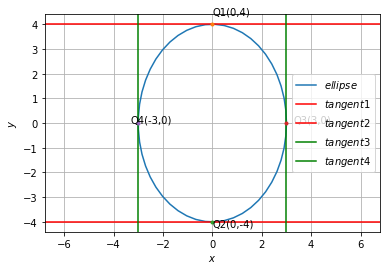
\includegraphics[width=\columnwidth]{./solutions/conics/1/16/ellipse.png}
	\caption{Figure depicting point of contact of tangents of ellipse parallel to x-axis and y-axis}
	\label{eq:solutions/1/16/fig1}
\end{figure}

\end{enumerate}
\item A chord of a circle is equal to the radius of the
circle. Find the angle subtended by the chord at
a point on the minor arc and also at a point on the
major arc.
\item If diagonals of a cyclic quadrilateral are diameters of the circle through the vertices of
the quadrilateral, prove that it is a rectangle.
\item If the non-parallel sides of a trapezium are equal, prove that it is cyclic.
\begin{enumerate}
\renewcommand{\theequation}{\theenumi}
\begin{enumerate}[label=\thesection.\arabic*.,ref=\thesection.\theenumi]
\numberwithin{equation}{enumi}

\item The vertices of $\triangle ABC$ are taken as follows:
\label{const:table1}
\\
\solution See Table. \ref{table:table1} 
%
\begin{table}[ht!]
\centering
%%%%%%%%%%%%%%%%%%%%%%%%%%%%%%%%%%%%%%%%%%%%%%%%%%%%%%%%%%%%%%%%%%%%%%
%%                                                                  %%
%%  This is the header of a LaTeX2e file exported from Gnumeric.    %%
%%                                                                  %%
%%  This file can be compiled as it stands or included in another   %%
%%  LaTeX document. The table is based on the longtable package so  %%
%%  the longtable options (headers, footers...) can be set in the   %%
%%  preamble section below (see PRAMBLE).                           %%
%%                                                                  %%
%%  To include the file in another, the following two lines must be %%
%%  in the including file:                                          %%
%%        \def\inputGnumericTable{}                                 %%
%%  at the beginning of the file and:                               %%
%%        \input{name-of-this-file.tex}                             %%
%%  where the table is to be placed. Note also that the including   %%
%%  file must use the following packages for the table to be        %%
%%  rendered correctly:                                             %%
%%    \usepackage[latin1]{inputenc}                                 %%
%%    \usepackage{color}                                            %%
%%    \usepackage{array}                                            %%
%%    \usepackage{longtable}                                        %%
%%    \usepackage{calc}                                             %%
%%    \usepackage{multirow}                                         %%
%%    \usepackage{hhline}                                           %%
%%    \usepackage{ifthen}                                           %%
%%  optionally (for landscape tables embedded in another document): %%
%%    \usepackage{lscape}                                           %%
%%                                                                  %%
%%%%%%%%%%%%%%%%%%%%%%%%%%%%%%%%%%%%%%%%%%%%%%%%%%%%%%%%%%%%%%%%%%%%%%



%%  This section checks if we are begin input into another file or  %%
%%  the file will be compiled alone. First use a macro taken from   %%
%%  the TeXbook ex 7.7 (suggestion of Han-Wen Nienhuys).            %%
\def\ifundefined#1{\expandafter\ifx\csname#1\endcsname\relax}


%%  Check for the \def token for inputed files. If it is not        %%
%%  defined, the file will be processed as a standalone and the     %%
%%  preamble will be used.                                          %%
\ifundefined{inputGnumericTable}

%%  We must be able to close or not the document at the end.        %%
	\def\gnumericTableEnd{\end{document}}


%%%%%%%%%%%%%%%%%%%%%%%%%%%%%%%%%%%%%%%%%%%%%%%%%%%%%%%%%%%%%%%%%%%%%%
%%                                                                  %%
%%  This is the PREAMBLE. Change these values to get the right      %%
%%  paper size and other niceties.                                  %%
%%                                                                  %%
%%%%%%%%%%%%%%%%%%%%%%%%%%%%%%%%%%%%%%%%%%%%%%%%%%%%%%%%%%%%%%%%%%%%%%

	\documentclass[12pt%
			  %,landscape%
                    ]{report}
       \usepackage[latin1]{inputenc}
       \usepackage{fullpage}
       \usepackage{color}
       \usepackage{array}
       \usepackage{longtable}
       \usepackage{calc}
       \usepackage{multirow}
       \usepackage{hhline}
       \usepackage{ifthen}

	\begin{document}


%%  End of the preamble for the standalone. The next section is for %%
%%  documents which are included into other LaTeX2e files.          %%
\else

%%  We are not a stand alone document. For a regular table, we will %%
%%  have no preamble and only define the closing to mean nothing.   %%
    \def\gnumericTableEnd{}

%%  If we want landscape mode in an embedded document, comment out  %%
%%  the line above and uncomment the two below. The table will      %%
%%  begin on a new page and run in landscape mode.                  %%
%       \def\gnumericTableEnd{\end{landscape}}
%       \begin{landscape}


%%  End of the else clause for this file being \input.              %%
\fi

%%%%%%%%%%%%%%%%%%%%%%%%%%%%%%%%%%%%%%%%%%%%%%%%%%%%%%%%%%%%%%%%%%%%%%
%%                                                                  %%
%%  The rest is the gnumeric table, except for the closing          %%
%%  statement. Changes below will alter the table's appearance.     %%
%%                                                                  %%
%%%%%%%%%%%%%%%%%%%%%%%%%%%%%%%%%%%%%%%%%%%%%%%%%%%%%%%%%%%%%%%%%%%%%%

\providecommand{\gnumericmathit}[1]{#1} 
%%  Uncomment the next line if you would like your numbers to be in %%
%%  italics if they are italizised in the gnumeric table.           %%
%\renewcommand{\gnumericmathit}[1]{\mathit{#1}}
\providecommand{\gnumericPB}[1]%
{\let\gnumericTemp=\\#1\let\\=\gnumericTemp\hspace{0pt}}
 \ifundefined{gnumericTableWidthDefined}
        \newlength{\gnumericTableWidth}
        \newlength{\gnumericTableWidthComplete}
        \newlength{\gnumericMultiRowLength}
        \global\def\gnumericTableWidthDefined{}
 \fi
%% The following setting protects this code from babel shorthands.  %%
 \ifthenelse{\isundefined{\languageshorthands}}{}{\languageshorthands{english}}
%%  The default table format retains the relative column widths of  %%
%%  gnumeric. They can easily be changed to c, r or l. In that case %%
%%  you may want to comment out the next line and uncomment the one %%
%%  thereafter                                                      %%
\providecommand\gnumbox{\makebox[0pt]}
%%\providecommand\gnumbox[1][]{\makebox}

%% to adjust positions in multirow situations                       %%
\setlength{\bigstrutjot}{\jot}
\setlength{\extrarowheight}{\doublerulesep}

%%  The \setlongtables command keeps column widths the same across  %%
%%  pages. Simply comment out next line for varying column widths.  %%
\setlongtables

\setlength\gnumericTableWidth{%
	53pt+%
	53pt+%
0pt}
\def\gumericNumCols{2}
\setlength\gnumericTableWidthComplete{\gnumericTableWidth+%
         \tabcolsep*\gumericNumCols*2+\arrayrulewidth*\gumericNumCols}
\ifthenelse{\lengthtest{\gnumericTableWidthComplete > \linewidth}}%
         {\def\gnumericScale{\ratio{\linewidth-%
                        \tabcolsep*\gumericNumCols*2-%
                        \arrayrulewidth*\gumericNumCols}%
{\gnumericTableWidth}}}%
{\def\gnumericScale{1}}

%%%%%%%%%%%%%%%%%%%%%%%%%%%%%%%%%%%%%%%%%%%%%%%%%%%%%%%%%%%%%%%%%%%%%%
%%                                                                  %%
%% The following are the widths of the various columns. We are      %%
%% defining them here because then they are easier to change.       %%
%% Depending on the cell formats we may use them more than once.    %%
%%                                                                  %%
%%%%%%%%%%%%%%%%%%%%%%%%%%%%%%%%%%%%%%%%%%%%%%%%%%%%%%%%%%%%%%%%%%%%%%

\ifthenelse{\isundefined{\gnumericColA}}{\newlength{\gnumericColA}}{}\settowidth{\gnumericColA}{\begin{tabular}{@{}p{53pt*\gnumericScale}@{}}x\end{tabular}}
\ifthenelse{\isundefined{\gnumericColB}}{\newlength{\gnumericColB}}{}\settowidth{\gnumericColB}{\begin{tabular}{@{}p{53pt*\gnumericScale}@{}}x\end{tabular}}

\begin{tabular}[c]{%
	b{\gnumericColA}%
	b{\gnumericColB}%
	}

%%%%%%%%%%%%%%%%%%%%%%%%%%%%%%%%%%%%%%%%%%%%%%%%%%%%%%%%%%%%%%%%%%%%%%
%%  The longtable options. (Caption, headers... see Goosens, p.124) %%
%	\caption{The Table Caption.}             \\	%
% \hline	% Across the top of the table.
%%  The rest of these options are table rows which are placed on    %%
%%  the first, last or every page. Use \multicolumn if you want.    %%

%%  Header for the first page.                                      %%
%	\multicolumn{2}{c}{The First Header} \\ \hline 
%	\multicolumn{1}{c}{colTag}	%Column 1
%	&\multicolumn{1}{c}{colTag}	\\ \hline %Last column
%	\endfirsthead

%%  The running header definition.                                  %%
%	\hline
%	\multicolumn{2}{l}{\ldots\small\slshape continued} \\ \hline
%	\multicolumn{1}{c}{colTag}	%Column 1
%	&\multicolumn{1}{c}{colTag}	\\ \hline %Last column
%	\endhead

%%  The running footer definition.                                  %%
%	\hline
%	\multicolumn{2}{r}{\small\slshape continued\ldots} \\
%	\endfoot

%%  The ending footer definition.                                   %%
%	\multicolumn{2}{c}{That's all folks} \\ \hline 
%	\endlastfoot
%%%%%%%%%%%%%%%%%%%%%%%%%%%%%%%%%%%%%%%%%%%%%%%%%%%%%%%%%%%%%%%%%%%%%%

\hhline{|--}
	 \multicolumn{2}{|p{	\gnumericColA+%
	\gnumericColB+%
	\tabcolsep*2*1}|}%
	{\gnumericPB{\centering}\gnumbox{\textbf{Initial Input Values}}}
\\
\hhline{|-|-|}
	 \multicolumn{1}{|p{\gnumericColA}|}%
	{\gnumericPB{\centering}\gnumbox{\textbf{Parameter}}}
	&\multicolumn{1}{p{\gnumericColB}|}%
	{\gnumericPB{\centering}\gnumbox{\textbf{Value}}}
\\
\hhline{|--|}
	 \multicolumn{1}{|p{\gnumericColA}|}%
	{\gnumericPB{\centering}\gnumbox{\textbf{a}}}
	&\multicolumn{1}{p{\gnumericColB}|}%
	{\gnumericPB{\centering}\gnumbox{\textbf{4}}}
\\
\hhline{|--|}
	 \multicolumn{1}{|p{\gnumericColA}|}%
	{\gnumericPB{\centering}\gnumbox{\textbf{b}}}
	&\multicolumn{1}{p{\gnumericColB}|}%
	{\gnumericPB{\centering}\gnumbox{\textbf{4}}}
\\
\hhline{|--|}
	 \multicolumn{1}{|p{\gnumericColA}|}%
	{\gnumericPB{\centering}\gnumbox{\textbf{c}}}
	&\multicolumn{1}{p{\gnumericColB}|}%
	{\gnumericPB{\centering}\gnumbox{\textbf{4}}}
\\
\hhline{|-|-|}
\end{tabular}

\ifthenelse{\isundefined{\languageshorthands}}{}{\languageshorthands{\languagename}}
\gnumericTableEnd

\caption{To construct triangle ABC}
\label{table:table1}	
\end{table}

%\item

\item The midpoints of sides are given as
\begin{align}
\vec{D} &= \frac{\vec{B}+\vec{C}}{2}
\label{eq:pointd}
\\
\vec{E} &= \frac{\vec{A}+\vec{C}}{2}
\\
\vec{F} &= \frac{\vec{A}+\vec{B}}{2}
\end{align}
\item Also Centroid divides median in ratio 2:1.So by section formulae $\vec{O}$ is given as
\begin{align}
\vec{O} &= \frac{2\vec{D}+\vec{A}}{3}
\label{eq:centr}
\end{align}

The derived coordinates are listed in \ref{table:table2}. 
%
\begin{table}[ht!]
\centering
%%%%%%%%%%%%%%%%%%%%%%%%%%%%%%%%%%%%%%%%%%%%%%%%%%%%%%%%%%%%%%%%%%%%%%
%%                                                                  %%
%%  This is the header of a LaTeX2e file exported from Gnumeric.    %%
%%                                                                  %%
%%  This file can be compiled as it stands or included in another   %%
%%  LaTeX document. The table is based on the longtable package so  %%
%%  the longtable options (headers, footers...) can be set in the   %%
%%  preamble section below (see PRAMBLE).                           %%
%%                                                                  %%
%%  To include the file in another, the following two lines must be %%
%%  in the including file:                                          %%
%%        \def\inputGnumericTable{}                                 %%
%%  at the beginning of the file and:                               %%
%%        \input{name-of-this-file.tex}                             %%
%%  where the table is to be placed. Note also that the including   %%
%%  file must use the following packages for the table to be        %%
%%  rendered correctly:                                             %%
%%    \usepackage[latin1]{inputenc}                                 %%
%%    \usepackage{color}                                            %%
%%    \usepackage{array}                                            %%
%%    \usepackage{longtable}                                        %%
%%    \usepackage{calc}                                             %%
%%    \usepackage{multirow}                                         %%
%%    \usepackage{hhline}                                           %%
%%    \usepackage{ifthen}                                           %%
%%  optionally (for landscape tables embedded in another document): %%
%%    \usepackage{lscape}                                           %%
%%                                                                  %%
%%%%%%%%%%%%%%%%%%%%%%%%%%%%%%%%%%%%%%%%%%%%%%%%%%%%%%%%%%%%%%%%%%%%%%



%%  This section checks if we are begin input into another file or  %%
%%  the file will be compiled alone. First use a macro taken from   %%
%%  the TeXbook ex 7.7 (suggestion of Han-Wen Nienhuys).            %%
\def\ifundefined#1{\expandafter\ifx\csname#1\endcsname\relax}


%%  Check for the \def token for inputed files. If it is not        %%
%%  defined, the file will be processed as a standalone and the     %%
%%  preamble will be used.                                          %%
\ifundefined{inputGnumericTable}

%%  We must be able to close or not the document at the end.        %%
	\def\gnumericTableEnd{\end{document}}


%%%%%%%%%%%%%%%%%%%%%%%%%%%%%%%%%%%%%%%%%%%%%%%%%%%%%%%%%%%%%%%%%%%%%%
%%                                                                  %%
%%  This is the PREAMBLE. Change these values to get the right      %%
%%  paper size and other niceties.                                  %%
%%                                                                  %%
%%%%%%%%%%%%%%%%%%%%%%%%%%%%%%%%%%%%%%%%%%%%%%%%%%%%%%%%%%%%%%%%%%%%%%

	\documentclass[12pt%
			  %,landscape%
                    ]{report}
       \usepackage[latin1]{inputenc}
       \usepackage{fullpage}
       \usepackage{color}
       \usepackage{array}
       \usepackage{longtable}
       \usepackage{calc}
       \usepackage{multirow}
       \usepackage{hhline}
       \usepackage{ifthen}

	\begin{document}


%%  End of the preamble for the standalone. The next section is for %%
%%  documents which are included into other LaTeX2e files.          %%
\else

%%  We are not a stand alone document. For a regular table, we will %%
%%  have no preamble and only define the closing to mean nothing.   %%
    \def\gnumericTableEnd{}

%%  If we want landscape mode in an embedded document, comment out  %%
%%  the line above and uncomment the two below. The table will      %%
%%  begin on a new page and run in landscape mode.                  %%
%       \def\gnumericTableEnd{\end{landscape}}
%       \begin{landscape}


%%  End of the else clause for this file being \input.              %%
\fi

%%%%%%%%%%%%%%%%%%%%%%%%%%%%%%%%%%%%%%%%%%%%%%%%%%%%%%%%%%%%%%%%%%%%%%
%%                                                                  %%
%%  The rest is the gnumeric table, except for the closing          %%
%%  statement. Changes below will alter the table's appearance.     %%
%%                                                                  %%
%%%%%%%%%%%%%%%%%%%%%%%%%%%%%%%%%%%%%%%%%%%%%%%%%%%%%%%%%%%%%%%%%%%%%%

\providecommand{\gnumericmathit}[1]{#1} 
%%  Uncomment the next line if you would like your numbers to be in %%
%%  italics if they are italizised in the gnumeric table.           %%
%\renewcommand{\gnumericmathit}[1]{\mathit{#1}}
\providecommand{\gnumericPB}[1]%
{\let\gnumericTemp=\\#1\let\\=\gnumericTemp\hspace{0pt}}
 \ifundefined{gnumericTableWidthDefined}
        \newlength{\gnumericTableWidth}
        \newlength{\gnumericTableWidthComplete}
        \newlength{\gnumericMultiRowLength}
        \global\def\gnumericTableWidthDefined{}
 \fi
%% The following setting protects this code from babel shorthands.  %%
 \ifthenelse{\isundefined{\languageshorthands}}{}{\languageshorthands{english}}
%%  The default table format retains the relative column widths of  %%
%%  gnumeric. They can easily be changed to c, r or l. In that case %%
%%  you may want to comment out the next line and uncomment the one %%
%%  thereafter                                                      %%
\providecommand\gnumbox{\makebox[0pt]}
%%\providecommand\gnumbox[1][]{\makebox}

%% to adjust positions in multirow situations                       %%
\setlength{\bigstrutjot}{\jot}
\setlength{\extrarowheight}{\doublerulesep}

%%  The \setlongtables command keeps column widths the same across  %%
%%  pages. Simply comment out next line for varying column widths.  %%
\setlongtables

\setlength\gnumericTableWidth{%
	50pt+%
	75pt+%
0pt}
\def\gumericNumCols{2}
\setlength\gnumericTableWidthComplete{\gnumericTableWidth+%
         \tabcolsep*\gumericNumCols*2+\arrayrulewidth*\gumericNumCols}
\ifthenelse{\lengthtest{\gnumericTableWidthComplete > \linewidth}}%
         {\def\gnumericScale{\ratio{\linewidth-%
                        \tabcolsep*\gumericNumCols*2-%
                        \arrayrulewidth*\gumericNumCols}%
{\gnumericTableWidth}}}%
{\def\gnumericScale{1}}

%%%%%%%%%%%%%%%%%%%%%%%%%%%%%%%%%%%%%%%%%%%%%%%%%%%%%%%%%%%%%%%%%%%%%%
%%                                                                  %%
%% The following are the widths of the various columns. We are      %%
%% defining them here because then they are easier to change.       %%
%% Depending on the cell formats we may use them more than once.    %%
%%                                                                  %%
%%%%%%%%%%%%%%%%%%%%%%%%%%%%%%%%%%%%%%%%%%%%%%%%%%%%%%%%%%%%%%%%%%%%%%

\ifthenelse{\isundefined{\gnumericColA}}{\newlength{\gnumericColA}}{}\settowidth{\gnumericColA}{\begin{tabular}{@{}p{50pt*\gnumericScale}@{}}x\end{tabular}}
\ifthenelse{\isundefined{\gnumericColB}}{\newlength{\gnumericColB}}{}\settowidth{\gnumericColB}{\begin{tabular}{@{}p{75pt*\gnumericScale}@{}}x\end{tabular}}

\begin{tabular}[c]{%
	b{\gnumericColA}%
	b{\gnumericColB}%
	}

%%%%%%%%%%%%%%%%%%%%%%%%%%%%%%%%%%%%%%%%%%%%%%%%%%%%%%%%%%%%%%%%%%%%%%
%%  The longtable options. (Caption, headers... see Goosens, p.124) %%
%	\caption{The Table Caption.}             \\	%
% \hline	% Across the top of the table.
%%  The rest of these options are table rows which are placed on    %%
%%  the first, last or every page. Use \multicolumn if you want.    %%

%%  Header for the first page.                                      %%
%	\multicolumn{2}{c}{The First Header} \\ \hline 
%	\multicolumn{1}{c}{colTag}	%Column 1
%	&\multicolumn{1}{c}{colTag}	\\ \hline %Last column
%	\endfirsthead

%%  The running header definition.                                  %%
%	\hline
%	\multicolumn{2}{l}{\ldots\small\slshape continued} \\ \hline
%	\multicolumn{1}{c}{colTag}	%Column 1
%	&\multicolumn{1}{c}{colTag}	\\ \hline %Last column
%	\endhead

%%  The running footer definition.                                  %%
%	\hline
%	\multicolumn{2}{r}{\small\slshape continued\ldots} \\
%	\endfoot

%%  The ending footer definition.                                   %%
%	\multicolumn{2}{c}{That's all folks} \\ \hline 
%	\endlastfoot
%%%%%%%%%%%%%%%%%%%%%%%%%%%%%%%%%%%%%%%%%%%%%%%%%%%%%%%%%%%%%%%%%%%%%%

\hhline{|-|-}
	 \multicolumn{1}{|p{\gnumericColA}|}%
	{\gnumericPB{\raggedright}\gnumbox[l]{Vector}}
	&\multicolumn{1}{p{\gnumericColB}|}%
	{\gnumericPB{\raggedright}\gnumbox[l]{Coordinates}}
\\
\hhline{|--|}
	 \multicolumn{1}{|p{\gnumericColA}|}%
	{\gnumericPB{\centering}\gnumbox{\textbf{D}}}
	&\multicolumn{1}{p{\gnumericColB}|}%
	{\gnumericPB{\centering}\gnumbox{$\myvec{3\\1}$}}
\\
\hhline{|--|}
	 \multicolumn{1}{|p{\gnumericColA}|}%
	{\gnumericPB{\centering}\gnumbox{\textbf{E}}}
	&\multicolumn{1}{p{\gnumericColB}|}%
	{\gnumericPB{\centering}\gnumbox{$\myvec{2\\0}$}}
\\
\hhline{|--|}
	 \multicolumn{1}{|p{\gnumericColA}|}%
	{\gnumericPB{\centering}\gnumbox{\textbf{F}}}
	&\multicolumn{1}{p{\gnumericColB}|}%
	{\gnumericPB{\centering}\gnumbox{$\myvec{1\\1}$}}
\\
\hhline{|--|}
	 \multicolumn{1}{|p{\gnumericColA}|}%
	{\gnumericPB{\centering}\gnumbox{\textbf{O}}}
	&\multicolumn{1}{p{\gnumericColB}|}%
	{\gnumericPB{\centering}\gnumbox{$\myvec{3\\\frac{2}{3}}$}}
\\
\hhline{|-|-|}
\end{tabular}

\ifthenelse{\isundefined{\languageshorthands}}{}{\languageshorthands{\languagename}}
\gnumericTableEnd

\caption{Derived coordinates of triangle ABC}
\label{table:table2}	
\end{table}

\end{enumerate}


General equation of conics is 
\begin{align}
    \vec{x}^T\vec{V}\vec{x}+ 2\vec{u}^T\vec{x}+f = 0
    \label{eq:solutions/1/16/eq:1}
\end{align}
Comparing with the equation given,
\begin{align}
\vec{V}=\myvec{\frac{1}{9} & 0 \\ 0 & \frac{1}{16}}\\
\vec{u}=\vec{0}\\
f=-1\\
\mydet{\vec{v}}=\mydet{\myvec{\frac{1}{9} & 0 \\ 0 & \frac{1}{16}}}>0
\end{align}
$\because \abs{\vec{V}}>0$, the given equation is of ellipse.\\
a)The tangents are parallel to the x-axis, hence, their direction and normal vectors, $\vec{m_1}$ and $\vec{n_1}$ are respectively,
\begin{align}
\vec{m_1}=\myvec{1\\0}\\
\vec{n_1}=\myvec{0\\1}
\end{align}
For an ellipse, given the normal vector $\vec{n}$, the tangent points of contact to the ellipse are given by
\begin{align}
    \vec{q}=\vec{V}^{-1}(\kappa \vec{n}-\vec{u})
    \label{eq:solutions/1/16/eq:2}
    =\vec{V}^{-1}\kappa \vec{n}
\end{align}
where
\begin{align}
    \kappa=\pm \sqrt{\frac{\vec{u^T}\vec{V}^{-1}\vec{u}-f}{\vec{n^T}\vec{V}^{-1}\vec{n}}}
    \label{eq:solutions/1/16/eq:2.0.9}\\
   =\pm \sqrt{\frac{-f}{\vec{n^T}\vec{V}^{-1}\vec{n}}}\\
    \vec{V}^{-1}=\myvec{9 & 0 \\ 0 & 16}\\
    \kappa_1=\pm \sqrt{\frac{-(-1)}{\myvec{0 & 1}\myvec{9 & 0 \\ 0 & 16} \myvec{0\\1}}}\\
 \implies \kappa_1=\pm \sqrt{\frac{1}{16}}\\
    \implies \kappa_1=\pm \frac{1}{4}      
\end{align}
From \eqref{eq:solutions/1/16/eq:2} , the point of contact $\vec{q_i}$ are,
\begin{align}
    \vec{q_1}=\myvec{9 & 0 \\ 0 & 16}\frac{1}{4}\myvec{0\\1}\\
    =\myvec{9 & 0 \\ 0 & 16}\myvec{0\\\frac{1}{4}}\\
    =\myvec{0\\4}\\
    \vec{q_2}=\myvec{9 & 0 \\ 0 & 16}\left(-\frac{1}{4}\right)\ \myvec{0\\1}\\
    =\myvec{9 & 0 \\ 0 & 16}\myvec{0\\-\frac{1}{4}}\\
    =\myvec{0\\-4}
\end{align}
b) The tangents are parallel to the y-axis, hence, their direction and normal vectors, $\vec{m_2}$ and $\vec{n_2}$ are respectively,
\begin{align}
\vec{m_2}=\myvec{0\\1}\\
\vec{n_2}=\myvec{1\\0}
\end{align}
Using equation \eqref{eq:solutions/1/16/eq:2.0.9}, the values of $\kappa$ for this case are
\begin{align}
     \kappa_2=\pm \sqrt{\frac{-(-1)}{\myvec{1 & 0}\myvec{9 & 0 \\ 0 & 16} \myvec{1\\0}}}\\
 \implies \kappa_2=\pm \sqrt{\frac{1}{9}}\\
    \implies \kappa_2=\pm \frac{1}{3} 
\end{align}
and from \eqref{eq:solutions/1/16/eq:2} , the point of contact $\vec{q_i}$ are,
\begin{align}
\vec{q_3}=\myvec{9 & 0 \\ 0 & 16}\frac{1}{3}\myvec{1\\0}\\
    =\myvec{9 & 0 \\ 0 & 16}\myvec{\frac{1}{3}\\0}\\
    =\myvec{3\\0}\\
\vec{q_4}=\myvec{9 & 0 \\ 0 & 16}\left(-\frac{1}{3}\right)\ \myvec{1\\0}\\
    =\myvec{9 & 0 \\ 0 & 16}\myvec{-\frac{1}{3}\\0}\\
    =\myvec{-3\\0}
\end{align}
 \begin{figure}[h!]
	\centering
	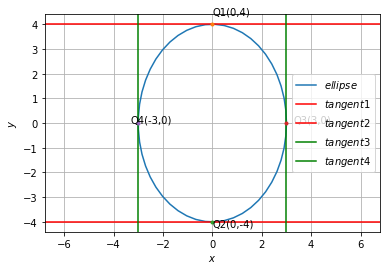
\includegraphics[width=\columnwidth]{./solutions/conics/1/16/ellipse.png}
	\caption{Figure depicting point of contact of tangents of ellipse parallel to x-axis and y-axis}
	\label{eq:solutions/1/16/fig1}
\end{figure}

\end{enumerate}

\item Two circles intersect at two points $B$ and $C$.
Through $B$, two line segments $ABD$ and $PBQ$
are drawn to intersect the circles at $A, D$ and $P$,
$Q$ respectively. Prove that
$\angle ACP = \angle QCD$.
\item If circles are drawn taking two sides of a triangle as diameters, prove that the point of
intersection of these circles lie on the third side.
\item $ABC$ and $ADC$ are two right triangles with common hypotenuse $AC$. Prove that
$\angle CAD = \angle CBD$.
\item Prove that a cyclic parallelogram is a rectangle.
\item Prove that the line of centres of two intersecting circles subtends equal angles at the
two points of intersection.
\item Let the vertex of an angle $ABC$ be located outside a circle and let the sides of the angle
intersect equal chords $AD$ and $CE$ with the circle. Prove that $\angle ABC$ is equal to half the
difference of the angles subtended by the chords $AC$ and $DE$ at the centre.
\begin{enumerate}
\renewcommand{\theequation}{\theenumi}
\begin{enumerate}[label=\thesection.\arabic*.,ref=\thesection.\theenumi]
\numberwithin{equation}{enumi}

\item The vertices of $\triangle ABC$ are taken as follows:
\label{const:table1}
\\
\solution See Table. \ref{table:table1} 
%
\begin{table}[ht!]
\centering
%%%%%%%%%%%%%%%%%%%%%%%%%%%%%%%%%%%%%%%%%%%%%%%%%%%%%%%%%%%%%%%%%%%%%%
%%                                                                  %%
%%  This is the header of a LaTeX2e file exported from Gnumeric.    %%
%%                                                                  %%
%%  This file can be compiled as it stands or included in another   %%
%%  LaTeX document. The table is based on the longtable package so  %%
%%  the longtable options (headers, footers...) can be set in the   %%
%%  preamble section below (see PRAMBLE).                           %%
%%                                                                  %%
%%  To include the file in another, the following two lines must be %%
%%  in the including file:                                          %%
%%        \def\inputGnumericTable{}                                 %%
%%  at the beginning of the file and:                               %%
%%        \input{name-of-this-file.tex}                             %%
%%  where the table is to be placed. Note also that the including   %%
%%  file must use the following packages for the table to be        %%
%%  rendered correctly:                                             %%
%%    \usepackage[latin1]{inputenc}                                 %%
%%    \usepackage{color}                                            %%
%%    \usepackage{array}                                            %%
%%    \usepackage{longtable}                                        %%
%%    \usepackage{calc}                                             %%
%%    \usepackage{multirow}                                         %%
%%    \usepackage{hhline}                                           %%
%%    \usepackage{ifthen}                                           %%
%%  optionally (for landscape tables embedded in another document): %%
%%    \usepackage{lscape}                                           %%
%%                                                                  %%
%%%%%%%%%%%%%%%%%%%%%%%%%%%%%%%%%%%%%%%%%%%%%%%%%%%%%%%%%%%%%%%%%%%%%%



%%  This section checks if we are begin input into another file or  %%
%%  the file will be compiled alone. First use a macro taken from   %%
%%  the TeXbook ex 7.7 (suggestion of Han-Wen Nienhuys).            %%
\def\ifundefined#1{\expandafter\ifx\csname#1\endcsname\relax}


%%  Check for the \def token for inputed files. If it is not        %%
%%  defined, the file will be processed as a standalone and the     %%
%%  preamble will be used.                                          %%
\ifundefined{inputGnumericTable}

%%  We must be able to close or not the document at the end.        %%
	\def\gnumericTableEnd{\end{document}}


%%%%%%%%%%%%%%%%%%%%%%%%%%%%%%%%%%%%%%%%%%%%%%%%%%%%%%%%%%%%%%%%%%%%%%
%%                                                                  %%
%%  This is the PREAMBLE. Change these values to get the right      %%
%%  paper size and other niceties.                                  %%
%%                                                                  %%
%%%%%%%%%%%%%%%%%%%%%%%%%%%%%%%%%%%%%%%%%%%%%%%%%%%%%%%%%%%%%%%%%%%%%%

	\documentclass[12pt%
			  %,landscape%
                    ]{report}
       \usepackage[latin1]{inputenc}
       \usepackage{fullpage}
       \usepackage{color}
       \usepackage{array}
       \usepackage{longtable}
       \usepackage{calc}
       \usepackage{multirow}
       \usepackage{hhline}
       \usepackage{ifthen}

	\begin{document}


%%  End of the preamble for the standalone. The next section is for %%
%%  documents which are included into other LaTeX2e files.          %%
\else

%%  We are not a stand alone document. For a regular table, we will %%
%%  have no preamble and only define the closing to mean nothing.   %%
    \def\gnumericTableEnd{}

%%  If we want landscape mode in an embedded document, comment out  %%
%%  the line above and uncomment the two below. The table will      %%
%%  begin on a new page and run in landscape mode.                  %%
%       \def\gnumericTableEnd{\end{landscape}}
%       \begin{landscape}


%%  End of the else clause for this file being \input.              %%
\fi

%%%%%%%%%%%%%%%%%%%%%%%%%%%%%%%%%%%%%%%%%%%%%%%%%%%%%%%%%%%%%%%%%%%%%%
%%                                                                  %%
%%  The rest is the gnumeric table, except for the closing          %%
%%  statement. Changes below will alter the table's appearance.     %%
%%                                                                  %%
%%%%%%%%%%%%%%%%%%%%%%%%%%%%%%%%%%%%%%%%%%%%%%%%%%%%%%%%%%%%%%%%%%%%%%

\providecommand{\gnumericmathit}[1]{#1} 
%%  Uncomment the next line if you would like your numbers to be in %%
%%  italics if they are italizised in the gnumeric table.           %%
%\renewcommand{\gnumericmathit}[1]{\mathit{#1}}
\providecommand{\gnumericPB}[1]%
{\let\gnumericTemp=\\#1\let\\=\gnumericTemp\hspace{0pt}}
 \ifundefined{gnumericTableWidthDefined}
        \newlength{\gnumericTableWidth}
        \newlength{\gnumericTableWidthComplete}
        \newlength{\gnumericMultiRowLength}
        \global\def\gnumericTableWidthDefined{}
 \fi
%% The following setting protects this code from babel shorthands.  %%
 \ifthenelse{\isundefined{\languageshorthands}}{}{\languageshorthands{english}}
%%  The default table format retains the relative column widths of  %%
%%  gnumeric. They can easily be changed to c, r or l. In that case %%
%%  you may want to comment out the next line and uncomment the one %%
%%  thereafter                                                      %%
\providecommand\gnumbox{\makebox[0pt]}
%%\providecommand\gnumbox[1][]{\makebox}

%% to adjust positions in multirow situations                       %%
\setlength{\bigstrutjot}{\jot}
\setlength{\extrarowheight}{\doublerulesep}

%%  The \setlongtables command keeps column widths the same across  %%
%%  pages. Simply comment out next line for varying column widths.  %%
\setlongtables

\setlength\gnumericTableWidth{%
	53pt+%
	53pt+%
0pt}
\def\gumericNumCols{2}
\setlength\gnumericTableWidthComplete{\gnumericTableWidth+%
         \tabcolsep*\gumericNumCols*2+\arrayrulewidth*\gumericNumCols}
\ifthenelse{\lengthtest{\gnumericTableWidthComplete > \linewidth}}%
         {\def\gnumericScale{\ratio{\linewidth-%
                        \tabcolsep*\gumericNumCols*2-%
                        \arrayrulewidth*\gumericNumCols}%
{\gnumericTableWidth}}}%
{\def\gnumericScale{1}}

%%%%%%%%%%%%%%%%%%%%%%%%%%%%%%%%%%%%%%%%%%%%%%%%%%%%%%%%%%%%%%%%%%%%%%
%%                                                                  %%
%% The following are the widths of the various columns. We are      %%
%% defining them here because then they are easier to change.       %%
%% Depending on the cell formats we may use them more than once.    %%
%%                                                                  %%
%%%%%%%%%%%%%%%%%%%%%%%%%%%%%%%%%%%%%%%%%%%%%%%%%%%%%%%%%%%%%%%%%%%%%%

\ifthenelse{\isundefined{\gnumericColA}}{\newlength{\gnumericColA}}{}\settowidth{\gnumericColA}{\begin{tabular}{@{}p{53pt*\gnumericScale}@{}}x\end{tabular}}
\ifthenelse{\isundefined{\gnumericColB}}{\newlength{\gnumericColB}}{}\settowidth{\gnumericColB}{\begin{tabular}{@{}p{53pt*\gnumericScale}@{}}x\end{tabular}}

\begin{tabular}[c]{%
	b{\gnumericColA}%
	b{\gnumericColB}%
	}

%%%%%%%%%%%%%%%%%%%%%%%%%%%%%%%%%%%%%%%%%%%%%%%%%%%%%%%%%%%%%%%%%%%%%%
%%  The longtable options. (Caption, headers... see Goosens, p.124) %%
%	\caption{The Table Caption.}             \\	%
% \hline	% Across the top of the table.
%%  The rest of these options are table rows which are placed on    %%
%%  the first, last or every page. Use \multicolumn if you want.    %%

%%  Header for the first page.                                      %%
%	\multicolumn{2}{c}{The First Header} \\ \hline 
%	\multicolumn{1}{c}{colTag}	%Column 1
%	&\multicolumn{1}{c}{colTag}	\\ \hline %Last column
%	\endfirsthead

%%  The running header definition.                                  %%
%	\hline
%	\multicolumn{2}{l}{\ldots\small\slshape continued} \\ \hline
%	\multicolumn{1}{c}{colTag}	%Column 1
%	&\multicolumn{1}{c}{colTag}	\\ \hline %Last column
%	\endhead

%%  The running footer definition.                                  %%
%	\hline
%	\multicolumn{2}{r}{\small\slshape continued\ldots} \\
%	\endfoot

%%  The ending footer definition.                                   %%
%	\multicolumn{2}{c}{That's all folks} \\ \hline 
%	\endlastfoot
%%%%%%%%%%%%%%%%%%%%%%%%%%%%%%%%%%%%%%%%%%%%%%%%%%%%%%%%%%%%%%%%%%%%%%

\hhline{|--}
	 \multicolumn{2}{|p{	\gnumericColA+%
	\gnumericColB+%
	\tabcolsep*2*1}|}%
	{\gnumericPB{\centering}\gnumbox{\textbf{Initial Input Values}}}
\\
\hhline{|-|-|}
	 \multicolumn{1}{|p{\gnumericColA}|}%
	{\gnumericPB{\centering}\gnumbox{\textbf{Parameter}}}
	&\multicolumn{1}{p{\gnumericColB}|}%
	{\gnumericPB{\centering}\gnumbox{\textbf{Value}}}
\\
\hhline{|--|}
	 \multicolumn{1}{|p{\gnumericColA}|}%
	{\gnumericPB{\centering}\gnumbox{\textbf{a}}}
	&\multicolumn{1}{p{\gnumericColB}|}%
	{\gnumericPB{\centering}\gnumbox{\textbf{4}}}
\\
\hhline{|--|}
	 \multicolumn{1}{|p{\gnumericColA}|}%
	{\gnumericPB{\centering}\gnumbox{\textbf{b}}}
	&\multicolumn{1}{p{\gnumericColB}|}%
	{\gnumericPB{\centering}\gnumbox{\textbf{4}}}
\\
\hhline{|--|}
	 \multicolumn{1}{|p{\gnumericColA}|}%
	{\gnumericPB{\centering}\gnumbox{\textbf{c}}}
	&\multicolumn{1}{p{\gnumericColB}|}%
	{\gnumericPB{\centering}\gnumbox{\textbf{4}}}
\\
\hhline{|-|-|}
\end{tabular}

\ifthenelse{\isundefined{\languageshorthands}}{}{\languageshorthands{\languagename}}
\gnumericTableEnd

\caption{To construct triangle ABC}
\label{table:table1}	
\end{table}

%\item

\item The midpoints of sides are given as
\begin{align}
\vec{D} &= \frac{\vec{B}+\vec{C}}{2}
\label{eq:pointd}
\\
\vec{E} &= \frac{\vec{A}+\vec{C}}{2}
\\
\vec{F} &= \frac{\vec{A}+\vec{B}}{2}
\end{align}
\item Also Centroid divides median in ratio 2:1.So by section formulae $\vec{O}$ is given as
\begin{align}
\vec{O} &= \frac{2\vec{D}+\vec{A}}{3}
\label{eq:centr}
\end{align}

The derived coordinates are listed in \ref{table:table2}. 
%
\begin{table}[ht!]
\centering
%%%%%%%%%%%%%%%%%%%%%%%%%%%%%%%%%%%%%%%%%%%%%%%%%%%%%%%%%%%%%%%%%%%%%%
%%                                                                  %%
%%  This is the header of a LaTeX2e file exported from Gnumeric.    %%
%%                                                                  %%
%%  This file can be compiled as it stands or included in another   %%
%%  LaTeX document. The table is based on the longtable package so  %%
%%  the longtable options (headers, footers...) can be set in the   %%
%%  preamble section below (see PRAMBLE).                           %%
%%                                                                  %%
%%  To include the file in another, the following two lines must be %%
%%  in the including file:                                          %%
%%        \def\inputGnumericTable{}                                 %%
%%  at the beginning of the file and:                               %%
%%        \input{name-of-this-file.tex}                             %%
%%  where the table is to be placed. Note also that the including   %%
%%  file must use the following packages for the table to be        %%
%%  rendered correctly:                                             %%
%%    \usepackage[latin1]{inputenc}                                 %%
%%    \usepackage{color}                                            %%
%%    \usepackage{array}                                            %%
%%    \usepackage{longtable}                                        %%
%%    \usepackage{calc}                                             %%
%%    \usepackage{multirow}                                         %%
%%    \usepackage{hhline}                                           %%
%%    \usepackage{ifthen}                                           %%
%%  optionally (for landscape tables embedded in another document): %%
%%    \usepackage{lscape}                                           %%
%%                                                                  %%
%%%%%%%%%%%%%%%%%%%%%%%%%%%%%%%%%%%%%%%%%%%%%%%%%%%%%%%%%%%%%%%%%%%%%%



%%  This section checks if we are begin input into another file or  %%
%%  the file will be compiled alone. First use a macro taken from   %%
%%  the TeXbook ex 7.7 (suggestion of Han-Wen Nienhuys).            %%
\def\ifundefined#1{\expandafter\ifx\csname#1\endcsname\relax}


%%  Check for the \def token for inputed files. If it is not        %%
%%  defined, the file will be processed as a standalone and the     %%
%%  preamble will be used.                                          %%
\ifundefined{inputGnumericTable}

%%  We must be able to close or not the document at the end.        %%
	\def\gnumericTableEnd{\end{document}}


%%%%%%%%%%%%%%%%%%%%%%%%%%%%%%%%%%%%%%%%%%%%%%%%%%%%%%%%%%%%%%%%%%%%%%
%%                                                                  %%
%%  This is the PREAMBLE. Change these values to get the right      %%
%%  paper size and other niceties.                                  %%
%%                                                                  %%
%%%%%%%%%%%%%%%%%%%%%%%%%%%%%%%%%%%%%%%%%%%%%%%%%%%%%%%%%%%%%%%%%%%%%%

	\documentclass[12pt%
			  %,landscape%
                    ]{report}
       \usepackage[latin1]{inputenc}
       \usepackage{fullpage}
       \usepackage{color}
       \usepackage{array}
       \usepackage{longtable}
       \usepackage{calc}
       \usepackage{multirow}
       \usepackage{hhline}
       \usepackage{ifthen}

	\begin{document}


%%  End of the preamble for the standalone. The next section is for %%
%%  documents which are included into other LaTeX2e files.          %%
\else

%%  We are not a stand alone document. For a regular table, we will %%
%%  have no preamble and only define the closing to mean nothing.   %%
    \def\gnumericTableEnd{}

%%  If we want landscape mode in an embedded document, comment out  %%
%%  the line above and uncomment the two below. The table will      %%
%%  begin on a new page and run in landscape mode.                  %%
%       \def\gnumericTableEnd{\end{landscape}}
%       \begin{landscape}


%%  End of the else clause for this file being \input.              %%
\fi

%%%%%%%%%%%%%%%%%%%%%%%%%%%%%%%%%%%%%%%%%%%%%%%%%%%%%%%%%%%%%%%%%%%%%%
%%                                                                  %%
%%  The rest is the gnumeric table, except for the closing          %%
%%  statement. Changes below will alter the table's appearance.     %%
%%                                                                  %%
%%%%%%%%%%%%%%%%%%%%%%%%%%%%%%%%%%%%%%%%%%%%%%%%%%%%%%%%%%%%%%%%%%%%%%

\providecommand{\gnumericmathit}[1]{#1} 
%%  Uncomment the next line if you would like your numbers to be in %%
%%  italics if they are italizised in the gnumeric table.           %%
%\renewcommand{\gnumericmathit}[1]{\mathit{#1}}
\providecommand{\gnumericPB}[1]%
{\let\gnumericTemp=\\#1\let\\=\gnumericTemp\hspace{0pt}}
 \ifundefined{gnumericTableWidthDefined}
        \newlength{\gnumericTableWidth}
        \newlength{\gnumericTableWidthComplete}
        \newlength{\gnumericMultiRowLength}
        \global\def\gnumericTableWidthDefined{}
 \fi
%% The following setting protects this code from babel shorthands.  %%
 \ifthenelse{\isundefined{\languageshorthands}}{}{\languageshorthands{english}}
%%  The default table format retains the relative column widths of  %%
%%  gnumeric. They can easily be changed to c, r or l. In that case %%
%%  you may want to comment out the next line and uncomment the one %%
%%  thereafter                                                      %%
\providecommand\gnumbox{\makebox[0pt]}
%%\providecommand\gnumbox[1][]{\makebox}

%% to adjust positions in multirow situations                       %%
\setlength{\bigstrutjot}{\jot}
\setlength{\extrarowheight}{\doublerulesep}

%%  The \setlongtables command keeps column widths the same across  %%
%%  pages. Simply comment out next line for varying column widths.  %%
\setlongtables

\setlength\gnumericTableWidth{%
	50pt+%
	75pt+%
0pt}
\def\gumericNumCols{2}
\setlength\gnumericTableWidthComplete{\gnumericTableWidth+%
         \tabcolsep*\gumericNumCols*2+\arrayrulewidth*\gumericNumCols}
\ifthenelse{\lengthtest{\gnumericTableWidthComplete > \linewidth}}%
         {\def\gnumericScale{\ratio{\linewidth-%
                        \tabcolsep*\gumericNumCols*2-%
                        \arrayrulewidth*\gumericNumCols}%
{\gnumericTableWidth}}}%
{\def\gnumericScale{1}}

%%%%%%%%%%%%%%%%%%%%%%%%%%%%%%%%%%%%%%%%%%%%%%%%%%%%%%%%%%%%%%%%%%%%%%
%%                                                                  %%
%% The following are the widths of the various columns. We are      %%
%% defining them here because then they are easier to change.       %%
%% Depending on the cell formats we may use them more than once.    %%
%%                                                                  %%
%%%%%%%%%%%%%%%%%%%%%%%%%%%%%%%%%%%%%%%%%%%%%%%%%%%%%%%%%%%%%%%%%%%%%%

\ifthenelse{\isundefined{\gnumericColA}}{\newlength{\gnumericColA}}{}\settowidth{\gnumericColA}{\begin{tabular}{@{}p{50pt*\gnumericScale}@{}}x\end{tabular}}
\ifthenelse{\isundefined{\gnumericColB}}{\newlength{\gnumericColB}}{}\settowidth{\gnumericColB}{\begin{tabular}{@{}p{75pt*\gnumericScale}@{}}x\end{tabular}}

\begin{tabular}[c]{%
	b{\gnumericColA}%
	b{\gnumericColB}%
	}

%%%%%%%%%%%%%%%%%%%%%%%%%%%%%%%%%%%%%%%%%%%%%%%%%%%%%%%%%%%%%%%%%%%%%%
%%  The longtable options. (Caption, headers... see Goosens, p.124) %%
%	\caption{The Table Caption.}             \\	%
% \hline	% Across the top of the table.
%%  The rest of these options are table rows which are placed on    %%
%%  the first, last or every page. Use \multicolumn if you want.    %%

%%  Header for the first page.                                      %%
%	\multicolumn{2}{c}{The First Header} \\ \hline 
%	\multicolumn{1}{c}{colTag}	%Column 1
%	&\multicolumn{1}{c}{colTag}	\\ \hline %Last column
%	\endfirsthead

%%  The running header definition.                                  %%
%	\hline
%	\multicolumn{2}{l}{\ldots\small\slshape continued} \\ \hline
%	\multicolumn{1}{c}{colTag}	%Column 1
%	&\multicolumn{1}{c}{colTag}	\\ \hline %Last column
%	\endhead

%%  The running footer definition.                                  %%
%	\hline
%	\multicolumn{2}{r}{\small\slshape continued\ldots} \\
%	\endfoot

%%  The ending footer definition.                                   %%
%	\multicolumn{2}{c}{That's all folks} \\ \hline 
%	\endlastfoot
%%%%%%%%%%%%%%%%%%%%%%%%%%%%%%%%%%%%%%%%%%%%%%%%%%%%%%%%%%%%%%%%%%%%%%

\hhline{|-|-}
	 \multicolumn{1}{|p{\gnumericColA}|}%
	{\gnumericPB{\raggedright}\gnumbox[l]{Vector}}
	&\multicolumn{1}{p{\gnumericColB}|}%
	{\gnumericPB{\raggedright}\gnumbox[l]{Coordinates}}
\\
\hhline{|--|}
	 \multicolumn{1}{|p{\gnumericColA}|}%
	{\gnumericPB{\centering}\gnumbox{\textbf{D}}}
	&\multicolumn{1}{p{\gnumericColB}|}%
	{\gnumericPB{\centering}\gnumbox{$\myvec{3\\1}$}}
\\
\hhline{|--|}
	 \multicolumn{1}{|p{\gnumericColA}|}%
	{\gnumericPB{\centering}\gnumbox{\textbf{E}}}
	&\multicolumn{1}{p{\gnumericColB}|}%
	{\gnumericPB{\centering}\gnumbox{$\myvec{2\\0}$}}
\\
\hhline{|--|}
	 \multicolumn{1}{|p{\gnumericColA}|}%
	{\gnumericPB{\centering}\gnumbox{\textbf{F}}}
	&\multicolumn{1}{p{\gnumericColB}|}%
	{\gnumericPB{\centering}\gnumbox{$\myvec{1\\1}$}}
\\
\hhline{|--|}
	 \multicolumn{1}{|p{\gnumericColA}|}%
	{\gnumericPB{\centering}\gnumbox{\textbf{O}}}
	&\multicolumn{1}{p{\gnumericColB}|}%
	{\gnumericPB{\centering}\gnumbox{$\myvec{3\\\frac{2}{3}}$}}
\\
\hhline{|-|-|}
\end{tabular}

\ifthenelse{\isundefined{\languageshorthands}}{}{\languageshorthands{\languagename}}
\gnumericTableEnd

\caption{Derived coordinates of triangle ABC}
\label{table:table2}	
\end{table}

\end{enumerate}


General equation of conics is 
\begin{align}
    \vec{x}^T\vec{V}\vec{x}+ 2\vec{u}^T\vec{x}+f = 0
    \label{eq:solutions/1/16/eq:1}
\end{align}
Comparing with the equation given,
\begin{align}
\vec{V}=\myvec{\frac{1}{9} & 0 \\ 0 & \frac{1}{16}}\\
\vec{u}=\vec{0}\\
f=-1\\
\mydet{\vec{v}}=\mydet{\myvec{\frac{1}{9} & 0 \\ 0 & \frac{1}{16}}}>0
\end{align}
$\because \abs{\vec{V}}>0$, the given equation is of ellipse.\\
a)The tangents are parallel to the x-axis, hence, their direction and normal vectors, $\vec{m_1}$ and $\vec{n_1}$ are respectively,
\begin{align}
\vec{m_1}=\myvec{1\\0}\\
\vec{n_1}=\myvec{0\\1}
\end{align}
For an ellipse, given the normal vector $\vec{n}$, the tangent points of contact to the ellipse are given by
\begin{align}
    \vec{q}=\vec{V}^{-1}(\kappa \vec{n}-\vec{u})
    \label{eq:solutions/1/16/eq:2}
    =\vec{V}^{-1}\kappa \vec{n}
\end{align}
where
\begin{align}
    \kappa=\pm \sqrt{\frac{\vec{u^T}\vec{V}^{-1}\vec{u}-f}{\vec{n^T}\vec{V}^{-1}\vec{n}}}
    \label{eq:solutions/1/16/eq:2.0.9}\\
   =\pm \sqrt{\frac{-f}{\vec{n^T}\vec{V}^{-1}\vec{n}}}\\
    \vec{V}^{-1}=\myvec{9 & 0 \\ 0 & 16}\\
    \kappa_1=\pm \sqrt{\frac{-(-1)}{\myvec{0 & 1}\myvec{9 & 0 \\ 0 & 16} \myvec{0\\1}}}\\
 \implies \kappa_1=\pm \sqrt{\frac{1}{16}}\\
    \implies \kappa_1=\pm \frac{1}{4}      
\end{align}
From \eqref{eq:solutions/1/16/eq:2} , the point of contact $\vec{q_i}$ are,
\begin{align}
    \vec{q_1}=\myvec{9 & 0 \\ 0 & 16}\frac{1}{4}\myvec{0\\1}\\
    =\myvec{9 & 0 \\ 0 & 16}\myvec{0\\\frac{1}{4}}\\
    =\myvec{0\\4}\\
    \vec{q_2}=\myvec{9 & 0 \\ 0 & 16}\left(-\frac{1}{4}\right)\ \myvec{0\\1}\\
    =\myvec{9 & 0 \\ 0 & 16}\myvec{0\\-\frac{1}{4}}\\
    =\myvec{0\\-4}
\end{align}
b) The tangents are parallel to the y-axis, hence, their direction and normal vectors, $\vec{m_2}$ and $\vec{n_2}$ are respectively,
\begin{align}
\vec{m_2}=\myvec{0\\1}\\
\vec{n_2}=\myvec{1\\0}
\end{align}
Using equation \eqref{eq:solutions/1/16/eq:2.0.9}, the values of $\kappa$ for this case are
\begin{align}
     \kappa_2=\pm \sqrt{\frac{-(-1)}{\myvec{1 & 0}\myvec{9 & 0 \\ 0 & 16} \myvec{1\\0}}}\\
 \implies \kappa_2=\pm \sqrt{\frac{1}{9}}\\
    \implies \kappa_2=\pm \frac{1}{3} 
\end{align}
and from \eqref{eq:solutions/1/16/eq:2} , the point of contact $\vec{q_i}$ are,
\begin{align}
\vec{q_3}=\myvec{9 & 0 \\ 0 & 16}\frac{1}{3}\myvec{1\\0}\\
    =\myvec{9 & 0 \\ 0 & 16}\myvec{\frac{1}{3}\\0}\\
    =\myvec{3\\0}\\
\vec{q_4}=\myvec{9 & 0 \\ 0 & 16}\left(-\frac{1}{3}\right)\ \myvec{1\\0}\\
    =\myvec{9 & 0 \\ 0 & 16}\myvec{-\frac{1}{3}\\0}\\
    =\myvec{-3\\0}
\end{align}
 \begin{figure}[h!]
	\centering
	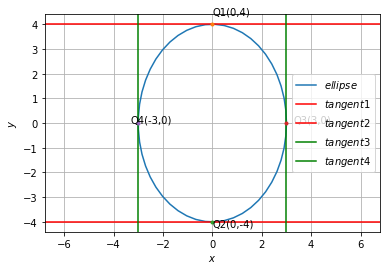
\includegraphics[width=\columnwidth]{./solutions/conics/1/16/ellipse.png}
	\caption{Figure depicting point of contact of tangents of ellipse parallel to x-axis and y-axis}
	\label{eq:solutions/1/16/fig1}
\end{figure}

\end{enumerate}

\item Prove that the circle drawn with any side of a rhombus as diameter, passes through
the point of intersection of its diagonals.
\item $ABCD$ is a parallelogram. The circle through $A, B$ and $C$ intersect $CD$ (produced if
necessary) at $E$. Prove that $AE = AD$.
\item $AC$ and $BD$ are chords of a circle which bisect each other. Prove that (i) $AC$ and $BD$ are
diameters, (ii) $ABCD$ is a rectangle.
\item Bisectors of angles $A, B$ and $C$ of a $\triangle ABC$ intersect its circumcircle at $D, E$ and
$F$ respectively. Prove that the angles of the $\triangle DEF$ are $90\degree – \frac{A}{2}, 90\degree – \frac{B}{2}$ and $90\degree – \frac{C}{2}$.
\item Two congruent circles intersect each other at points A and B. Through A any line segment PAQ is drawn so that $P, Q$ lie on the two circles. Prove that $BP = BQ$.
\item In any $\triangle ABC$, if the angle bisector of $\angle A$ and perpendicular bisector of $BC$ intersect, prove that they intersect on the circumcircle of the $\triangle ABC$.
%
\item The lengths of tangents drawn from an external point to a circle are equal.
%
\item Prove that in two concentric circles, the chord of the larger circle, which touches the smaller circle, is bisected at the point of contact.
%
\item Two tangents $TP$ and $TQ$ are drawn to a circle with centre $O$ from an external point $T$. Prove that $\angle PTQ = 2 \angle OPQ$.
%
\item Prove that the tangents drawn at the ends of a diameter of a circle are parallel. 
\item  Prove that the perpendicular at the point of contact to the tangent to a circle passes through the centre.
\item A quadrilateral $ABCD$ is drawn to circumscribe a circle. Prove that 
$AB + CD = AD + BC$.
%
\item $XY$ and $X'Y'$ are two parallel tangents to a circle with centre $O$ and another tangent $AB$ with point of contact $C$ intersecting $XY$ at $A$ and $X'Y'$ at $B$. Prove that $\angle AOB = 90\degree$
\item Prove that the angle between the two tangents drawn from an external point to a circle is supplementary to the angle subtended by the line-segment joining the points of contact at the centre.
\item  Prove that the parallelogram circumscribing a circle is a rhombus.
%
\item Prove that opposite sides of a quadrilateral circumscribing a circle subtend supplementary angles at the centre of the circle.
%
\item Find the area of a sector of angle $p$ (in degrees) of a circle with radius $R$. 
\item  Two chords $AB$ and $CD$ intersect each other at the point $P$. Prove that : 
\begin{enumerate}
\item   $\triangle  APC  \sim   \triangle  DPB$
\item  $AP . PB = CP . DP$
\end{enumerate}
\item Two chords $AB$ and $CD$ of a circle intersect each other at the point $P$ (when produced) outside the circle. Prove that 
\begin{enumerate}
\item   $\triangle  PAC  \sim   \triangle  PDB$
\item  $PA . PB = PC . PD$
\end{enumerate}

\end{enumerate}
